% Project report in the ICLR 2025 conference format (official style files in this folder).
\documentclass{article}
\usepackage{iclr2025_conference,times}

% Optional math commands from https://github.com/goodfeli/dlbook_notation.
%%%%% NEW MATH DEFINITIONS %%%%%

\usepackage{amsmath,amsfonts,bm}

% Mark sections of captions for referring to divisions of figures
\newcommand{\figleft}{{\em (Left)}}
\newcommand{\figcenter}{{\em (Center)}}
\newcommand{\figright}{{\em (Right)}}
\newcommand{\figtop}{{\em (Top)}}
\newcommand{\figbottom}{{\em (Bottom)}}
\newcommand{\captiona}{{\em (a)}}
\newcommand{\captionb}{{\em (b)}}
\newcommand{\captionc}{{\em (c)}}
\newcommand{\captiond}{{\em (d)}}

% Highlight a newly defined term
\newcommand{\newterm}[1]{{\bf #1}}


% Figure reference, lower-case.
\def\figref#1{figure~\ref{#1}}
% Figure reference, capital. For start of sentence
\def\Figref#1{Figure~\ref{#1}}
\def\twofigref#1#2{figures \ref{#1} and \ref{#2}}
\def\quadfigref#1#2#3#4{figures \ref{#1}, \ref{#2}, \ref{#3} and \ref{#4}}
% Section reference, lower-case.
\def\secref#1{section~\ref{#1}}
% Section reference, capital.
\def\Secref#1{Section~\ref{#1}}
% Reference to two sections.
\def\twosecrefs#1#2{sections \ref{#1} and \ref{#2}}
% Reference to three sections.
\def\secrefs#1#2#3{sections \ref{#1}, \ref{#2} and \ref{#3}}
% Reference to an equation, lower-case.
\def\eqref#1{equation~\ref{#1}}
% Reference to an equation, upper case
\def\Eqref#1{Equation~\ref{#1}}
% A raw reference to an equation---avoid using if possible
\def\plaineqref#1{\ref{#1}}
% Reference to a chapter, lower-case.
\def\chapref#1{chapter~\ref{#1}}
% Reference to an equation, upper case.
\def\Chapref#1{Chapter~\ref{#1}}
% Reference to a range of chapters
\def\rangechapref#1#2{chapters\ref{#1}--\ref{#2}}
% Reference to an algorithm, lower-case.
\def\algref#1{algorithm~\ref{#1}}
% Reference to an algorithm, upper case.
\def\Algref#1{Algorithm~\ref{#1}}
\def\twoalgref#1#2{algorithms \ref{#1} and \ref{#2}}
\def\Twoalgref#1#2{Algorithms \ref{#1} and \ref{#2}}
% Reference to a part, lower case
\def\partref#1{part~\ref{#1}}
% Reference to a part, upper case
\def\Partref#1{Part~\ref{#1}}
\def\twopartref#1#2{parts \ref{#1} and \ref{#2}}

\def\ceil#1{\lceil #1 \rceil}
\def\floor#1{\lfloor #1 \rfloor}
\def\1{\bm{1}}
\newcommand{\train}{\mathcal{D}}
\newcommand{\valid}{\mathcal{D_{\mathrm{valid}}}}
\newcommand{\test}{\mathcal{D_{\mathrm{test}}}}

\def\eps{{\epsilon}}


% Random variables
\def\reta{{\textnormal{$\eta$}}}
\def\ra{{\textnormal{a}}}
\def\rb{{\textnormal{b}}}
\def\rc{{\textnormal{c}}}
\def\rd{{\textnormal{d}}}
\def\re{{\textnormal{e}}}
\def\rf{{\textnormal{f}}}
\def\rg{{\textnormal{g}}}
\def\rh{{\textnormal{h}}}
\def\ri{{\textnormal{i}}}
\def\rj{{\textnormal{j}}}
\def\rk{{\textnormal{k}}}
\def\rl{{\textnormal{l}}}
% rm is already a command, just don't name any random variables m
\def\rn{{\textnormal{n}}}
\def\ro{{\textnormal{o}}}
\def\rp{{\textnormal{p}}}
\def\rq{{\textnormal{q}}}
\def\rr{{\textnormal{r}}}
\def\rs{{\textnormal{s}}}
\def\rt{{\textnormal{t}}}
\def\ru{{\textnormal{u}}}
\def\rv{{\textnormal{v}}}
\def\rw{{\textnormal{w}}}
\def\rx{{\textnormal{x}}}
\def\ry{{\textnormal{y}}}
\def\rz{{\textnormal{z}}}

% Random vectors
\def\rvepsilon{{\mathbf{\epsilon}}}
\def\rvtheta{{\mathbf{\theta}}}
\def\rva{{\mathbf{a}}}
\def\rvb{{\mathbf{b}}}
\def\rvc{{\mathbf{c}}}
\def\rvd{{\mathbf{d}}}
\def\rve{{\mathbf{e}}}
\def\rvf{{\mathbf{f}}}
\def\rvg{{\mathbf{g}}}
\def\rvh{{\mathbf{h}}}
\def\rvu{{\mathbf{i}}}
\def\rvj{{\mathbf{j}}}
\def\rvk{{\mathbf{k}}}
\def\rvl{{\mathbf{l}}}
\def\rvm{{\mathbf{m}}}
\def\rvn{{\mathbf{n}}}
\def\rvo{{\mathbf{o}}}
\def\rvp{{\mathbf{p}}}
\def\rvq{{\mathbf{q}}}
\def\rvr{{\mathbf{r}}}
\def\rvs{{\mathbf{s}}}
\def\rvt{{\mathbf{t}}}
\def\rvu{{\mathbf{u}}}
\def\rvv{{\mathbf{v}}}
\def\rvw{{\mathbf{w}}}
\def\rvx{{\mathbf{x}}}
\def\rvy{{\mathbf{y}}}
\def\rvz{{\mathbf{z}}}

% Elements of random vectors
\def\erva{{\textnormal{a}}}
\def\ervb{{\textnormal{b}}}
\def\ervc{{\textnormal{c}}}
\def\ervd{{\textnormal{d}}}
\def\erve{{\textnormal{e}}}
\def\ervf{{\textnormal{f}}}
\def\ervg{{\textnormal{g}}}
\def\ervh{{\textnormal{h}}}
\def\ervi{{\textnormal{i}}}
\def\ervj{{\textnormal{j}}}
\def\ervk{{\textnormal{k}}}
\def\ervl{{\textnormal{l}}}
\def\ervm{{\textnormal{m}}}
\def\ervn{{\textnormal{n}}}
\def\ervo{{\textnormal{o}}}
\def\ervp{{\textnormal{p}}}
\def\ervq{{\textnormal{q}}}
\def\ervr{{\textnormal{r}}}
\def\ervs{{\textnormal{s}}}
\def\ervt{{\textnormal{t}}}
\def\ervu{{\textnormal{u}}}
\def\ervv{{\textnormal{v}}}
\def\ervw{{\textnormal{w}}}
\def\ervx{{\textnormal{x}}}
\def\ervy{{\textnormal{y}}}
\def\ervz{{\textnormal{z}}}

% Random matrices
\def\rmA{{\mathbf{A}}}
\def\rmB{{\mathbf{B}}}
\def\rmC{{\mathbf{C}}}
\def\rmD{{\mathbf{D}}}
\def\rmE{{\mathbf{E}}}
\def\rmF{{\mathbf{F}}}
\def\rmG{{\mathbf{G}}}
\def\rmH{{\mathbf{H}}}
\def\rmI{{\mathbf{I}}}
\def\rmJ{{\mathbf{J}}}
\def\rmK{{\mathbf{K}}}
\def\rmL{{\mathbf{L}}}
\def\rmM{{\mathbf{M}}}
\def\rmN{{\mathbf{N}}}
\def\rmO{{\mathbf{O}}}
\def\rmP{{\mathbf{P}}}
\def\rmQ{{\mathbf{Q}}}
\def\rmR{{\mathbf{R}}}
\def\rmS{{\mathbf{S}}}
\def\rmT{{\mathbf{T}}}
\def\rmU{{\mathbf{U}}}
\def\rmV{{\mathbf{V}}}
\def\rmW{{\mathbf{W}}}
\def\rmX{{\mathbf{X}}}
\def\rmY{{\mathbf{Y}}}
\def\rmZ{{\mathbf{Z}}}

% Elements of random matrices
\def\ermA{{\textnormal{A}}}
\def\ermB{{\textnormal{B}}}
\def\ermC{{\textnormal{C}}}
\def\ermD{{\textnormal{D}}}
\def\ermE{{\textnormal{E}}}
\def\ermF{{\textnormal{F}}}
\def\ermG{{\textnormal{G}}}
\def\ermH{{\textnormal{H}}}
\def\ermI{{\textnormal{I}}}
\def\ermJ{{\textnormal{J}}}
\def\ermK{{\textnormal{K}}}
\def\ermL{{\textnormal{L}}}
\def\ermM{{\textnormal{M}}}
\def\ermN{{\textnormal{N}}}
\def\ermO{{\textnormal{O}}}
\def\ermP{{\textnormal{P}}}
\def\ermQ{{\textnormal{Q}}}
\def\ermR{{\textnormal{R}}}
\def\ermS{{\textnormal{S}}}
\def\ermT{{\textnormal{T}}}
\def\ermU{{\textnormal{U}}}
\def\ermV{{\textnormal{V}}}
\def\ermW{{\textnormal{W}}}
\def\ermX{{\textnormal{X}}}
\def\ermY{{\textnormal{Y}}}
\def\ermZ{{\textnormal{Z}}}

% Vectors
\def\vzero{{\bm{0}}}
\def\vone{{\bm{1}}}
\def\vmu{{\bm{\mu}}}
\def\vtheta{{\bm{\theta}}}
\def\va{{\bm{a}}}
\def\vb{{\bm{b}}}
\def\vc{{\bm{c}}}
\def\vd{{\bm{d}}}
\def\ve{{\bm{e}}}
\def\vf{{\bm{f}}}
\def\vg{{\bm{g}}}
\def\vh{{\bm{h}}}
\def\vi{{\bm{i}}}
\def\vj{{\bm{j}}}
\def\vk{{\bm{k}}}
\def\vl{{\bm{l}}}
\def\vm{{\bm{m}}}
\def\vn{{\bm{n}}}
\def\vo{{\bm{o}}}
\def\vp{{\bm{p}}}
\def\vq{{\bm{q}}}
\def\vr{{\bm{r}}}
\def\vs{{\bm{s}}}
\def\vt{{\bm{t}}}
\def\vu{{\bm{u}}}
\def\vv{{\bm{v}}}
\def\vw{{\bm{w}}}
\def\vx{{\bm{x}}}
\def\vy{{\bm{y}}}
\def\vz{{\bm{z}}}

% Elements of vectors
\def\evalpha{{\alpha}}
\def\evbeta{{\beta}}
\def\evepsilon{{\epsilon}}
\def\evlambda{{\lambda}}
\def\evomega{{\omega}}
\def\evmu{{\mu}}
\def\evpsi{{\psi}}
\def\evsigma{{\sigma}}
\def\evtheta{{\theta}}
\def\eva{{a}}
\def\evb{{b}}
\def\evc{{c}}
\def\evd{{d}}
\def\eve{{e}}
\def\evf{{f}}
\def\evg{{g}}
\def\evh{{h}}
\def\evi{{i}}
\def\evj{{j}}
\def\evk{{k}}
\def\evl{{l}}
\def\evm{{m}}
\def\evn{{n}}
\def\evo{{o}}
\def\evp{{p}}
\def\evq{{q}}
\def\evr{{r}}
\def\evs{{s}}
\def\evt{{t}}
\def\evu{{u}}
\def\evv{{v}}
\def\evw{{w}}
\def\evx{{x}}
\def\evy{{y}}
\def\evz{{z}}

% Matrix
\def\mA{{\bm{A}}}
\def\mB{{\bm{B}}}
\def\mC{{\bm{C}}}
\def\mD{{\bm{D}}}
\def\mE{{\bm{E}}}
\def\mF{{\bm{F}}}
\def\mG{{\bm{G}}}
\def\mH{{\bm{H}}}
\def\mI{{\bm{I}}}
\def\mJ{{\bm{J}}}
\def\mK{{\bm{K}}}
\def\mL{{\bm{L}}}
\def\mM{{\bm{M}}}
\def\mN{{\bm{N}}}
\def\mO{{\bm{O}}}
\def\mP{{\bm{P}}}
\def\mQ{{\bm{Q}}}
\def\mR{{\bm{R}}}
\def\mS{{\bm{S}}}
\def\mT{{\bm{T}}}
\def\mU{{\bm{U}}}
\def\mV{{\bm{V}}}
\def\mW{{\bm{W}}}
\def\mX{{\bm{X}}}
\def\mY{{\bm{Y}}}
\def\mZ{{\bm{Z}}}
\def\mBeta{{\bm{\beta}}}
\def\mPhi{{\bm{\Phi}}}
\def\mLambda{{\bm{\Lambda}}}
\def\mSigma{{\bm{\Sigma}}}

% Tensor
\DeclareMathAlphabet{\mathsfit}{\encodingdefault}{\sfdefault}{m}{sl}
\SetMathAlphabet{\mathsfit}{bold}{\encodingdefault}{\sfdefault}{bx}{n}
\newcommand{\tens}[1]{\bm{\mathsfit{#1}}}
\def\tA{{\tens{A}}}
\def\tB{{\tens{B}}}
\def\tC{{\tens{C}}}
\def\tD{{\tens{D}}}
\def\tE{{\tens{E}}}
\def\tF{{\tens{F}}}
\def\tG{{\tens{G}}}
\def\tH{{\tens{H}}}
\def\tI{{\tens{I}}}
\def\tJ{{\tens{J}}}
\def\tK{{\tens{K}}}
\def\tL{{\tens{L}}}
\def\tM{{\tens{M}}}
\def\tN{{\tens{N}}}
\def\tO{{\tens{O}}}
\def\tP{{\tens{P}}}
\def\tQ{{\tens{Q}}}
\def\tR{{\tens{R}}}
\def\tS{{\tens{S}}}
\def\tT{{\tens{T}}}
\def\tU{{\tens{U}}}
\def\tV{{\tens{V}}}
\def\tW{{\tens{W}}}
\def\tX{{\tens{X}}}
\def\tY{{\tens{Y}}}
\def\tZ{{\tens{Z}}}


% Graph
\def\gA{{\mathcal{A}}}
\def\gB{{\mathcal{B}}}
\def\gC{{\mathcal{C}}}
\def\gD{{\mathcal{D}}}
\def\gE{{\mathcal{E}}}
\def\gF{{\mathcal{F}}}
\def\gG{{\mathcal{G}}}
\def\gH{{\mathcal{H}}}
\def\gI{{\mathcal{I}}}
\def\gJ{{\mathcal{J}}}
\def\gK{{\mathcal{K}}}
\def\gL{{\mathcal{L}}}
\def\gM{{\mathcal{M}}}
\def\gN{{\mathcal{N}}}
\def\gO{{\mathcal{O}}}
\def\gP{{\mathcal{P}}}
\def\gQ{{\mathcal{Q}}}
\def\gR{{\mathcal{R}}}
\def\gS{{\mathcal{S}}}
\def\gT{{\mathcal{T}}}
\def\gU{{\mathcal{U}}}
\def\gV{{\mathcal{V}}}
\def\gW{{\mathcal{W}}}
\def\gX{{\mathcal{X}}}
\def\gY{{\mathcal{Y}}}
\def\gZ{{\mathcal{Z}}}

% Sets
\def\sA{{\mathbb{A}}}
\def\sB{{\mathbb{B}}}
\def\sC{{\mathbb{C}}}
\def\sD{{\mathbb{D}}}
% Don't use a set called E, because this would be the same as our symbol
% for expectation.
\def\sF{{\mathbb{F}}}
\def\sG{{\mathbb{G}}}
\def\sH{{\mathbb{H}}}
\def\sI{{\mathbb{I}}}
\def\sJ{{\mathbb{J}}}
\def\sK{{\mathbb{K}}}
\def\sL{{\mathbb{L}}}
\def\sM{{\mathbb{M}}}
\def\sN{{\mathbb{N}}}
\def\sO{{\mathbb{O}}}
\def\sP{{\mathbb{P}}}
\def\sQ{{\mathbb{Q}}}
\def\sR{{\mathbb{R}}}
\def\sS{{\mathbb{S}}}
\def\sT{{\mathbb{T}}}
\def\sU{{\mathbb{U}}}
\def\sV{{\mathbb{V}}}
\def\sW{{\mathbb{W}}}
\def\sX{{\mathbb{X}}}
\def\sY{{\mathbb{Y}}}
\def\sZ{{\mathbb{Z}}}

% Entries of a matrix
\def\emLambda{{\Lambda}}
\def\emA{{A}}
\def\emB{{B}}
\def\emC{{C}}
\def\emD{{D}}
\def\emE{{E}}
\def\emF{{F}}
\def\emG{{G}}
\def\emH{{H}}
\def\emI{{I}}
\def\emJ{{J}}
\def\emK{{K}}
\def\emL{{L}}
\def\emM{{M}}
\def\emN{{N}}
\def\emO{{O}}
\def\emP{{P}}
\def\emQ{{Q}}
\def\emR{{R}}
\def\emS{{S}}
\def\emT{{T}}
\def\emU{{U}}
\def\emV{{V}}
\def\emW{{W}}
\def\emX{{X}}
\def\emY{{Y}}
\def\emZ{{Z}}
\def\emSigma{{\Sigma}}

% entries of a tensor
% Same font as tensor, without \bm wrapper
\newcommand{\etens}[1]{\mathsfit{#1}}
\def\etLambda{{\etens{\Lambda}}}
\def\etA{{\etens{A}}}
\def\etB{{\etens{B}}}
\def\etC{{\etens{C}}}
\def\etD{{\etens{D}}}
\def\etE{{\etens{E}}}
\def\etF{{\etens{F}}}
\def\etG{{\etens{G}}}
\def\etH{{\etens{H}}}
\def\etI{{\etens{I}}}
\def\etJ{{\etens{J}}}
\def\etK{{\etens{K}}}
\def\etL{{\etens{L}}}
\def\etM{{\etens{M}}}
\def\etN{{\etens{N}}}
\def\etO{{\etens{O}}}
\def\etP{{\etens{P}}}
\def\etQ{{\etens{Q}}}
\def\etR{{\etens{R}}}
\def\etS{{\etens{S}}}
\def\etT{{\etens{T}}}
\def\etU{{\etens{U}}}
\def\etV{{\etens{V}}}
\def\etW{{\etens{W}}}
\def\etX{{\etens{X}}}
\def\etY{{\etens{Y}}}
\def\etZ{{\etens{Z}}}

% The true underlying data generating distribution
\newcommand{\pdata}{p_{\rm{data}}}
% The empirical distribution defined by the training set
\newcommand{\ptrain}{\hat{p}_{\rm{data}}}
\newcommand{\Ptrain}{\hat{P}_{\rm{data}}}
% The model distribution
\newcommand{\pmodel}{p_{\rm{model}}}
\newcommand{\Pmodel}{P_{\rm{model}}}
\newcommand{\ptildemodel}{\tilde{p}_{\rm{model}}}
% Stochastic autoencoder distributions
\newcommand{\pencode}{p_{\rm{encoder}}}
\newcommand{\pdecode}{p_{\rm{decoder}}}
\newcommand{\precons}{p_{\rm{reconstruct}}}

\newcommand{\laplace}{\mathrm{Laplace}} % Laplace distribution

\newcommand{\E}{\mathbb{E}}
\newcommand{\Ls}{\mathcal{L}}
\newcommand{\R}{\mathbb{R}}
\newcommand{\emp}{\tilde{p}}
\newcommand{\lr}{\alpha}
\newcommand{\reg}{\lambda}
\newcommand{\rect}{\mathrm{rectifier}}
\newcommand{\softmax}{\mathrm{softmax}}
\newcommand{\sigmoid}{\sigma}
\newcommand{\softplus}{\zeta}
\newcommand{\KL}{D_{\mathrm{KL}}}
\newcommand{\Var}{\mathrm{Var}}
\newcommand{\standarderror}{\mathrm{SE}}
\newcommand{\Cov}{\mathrm{Cov}}
% Wolfram Mathworld says $L^2$ is for function spaces and $\ell^2$ is for vectors
% But then they seem to use $L^2$ for vectors throughout the site, and so does
% wikipedia.
\newcommand{\normlzero}{L^0}
\newcommand{\normlone}{L^1}
\newcommand{\normltwo}{L^2}
\newcommand{\normlp}{L^p}
\newcommand{\normmax}{L^\infty}

\newcommand{\parents}{Pa} % See usage in notation.tex. Chosen to match Daphne's book.

\DeclareMathOperator*{\argmax}{arg\,max}
\DeclareMathOperator*{\argmin}{arg\,min}

\DeclareMathOperator{\sign}{sign}
\DeclareMathOperator{\Tr}{Tr}
\let\ab\allowbreak


\usepackage[T1]{fontenc}
\usepackage[utf8]{inputenc}
\usepackage{hyperref}
\usepackage{url}
\usepackage{graphicx}
\usepackage{booktabs}
\usepackage{multirow}
\usepackage{adjustbox}
\usepackage{float}
\usepackage{subcaption}
\usepackage{placeins}
\usepackage{titletoc}  % partial table of contents for the appendix

\hypersetup{colorlinks=true, linkcolor=blue!50!black, citecolor=blue!50!black, urlcolor=blue!50!black}

\title{Classifying Cardiac Pathologies \\ from MRI Segmentations, Revisited}

\author{Noé Mosca \\
Télécom Paris, Institut Polytechnique de Paris}

\iclrfinalcopy % show the authors
\begin{document}

\maketitle
% The style prints a conference banner in the header; this is a course project report.
\lhead{IMA205 challenge report, Télécom Paris}

\begin{abstract}
We classify 150 patients of the ACDC dataset into five diagnostic groups (normal, myocardial infarction, dilated and hypertrophic cardiomyopathy, abnormal right ventricle) from segmentations of their end-diastolic and end-systolic cardiac MRI, height and weight. The 100 training patients are labeled; in the 50 test patients, the left-ventricular (LV) cavity is not segmented and must be reconstructed. With so few patients, the evaluation protocol matters as much as the model. On 21 classical volumetric biomarkers, selecting the hyper-parameters of standard classifiers on a single cross-validation split and reporting the best score gives accuracies of 0.91 to 0.95; nested cross-validation repeated over several splits gives 0.90 to 0.94 for the same models and grids, and an ensemble weight chosen on the evaluation folds varies from 0 to 0.9 with the random seed. Filling the holes of the myocardium recovers the LV cavity with a mean Dice of 0.997; a convex-hull fallback on the few slices where the myocardial ring is open brings it to 0.9998, and training on reconstructed or true cavities makes no measurable difference. What does improve classification is describing the myocardial wall: 11 thickness features raise the accuracy of linear models and of an ensemble of 50 MLPs by 3 to 6 points. The final model, an average of this ensemble and a linear SVM, reaches $0.966 \pm 0.011$ in nested cross-validation; its remaining errors are infarcted hearts that look dilated, and conversely.
\end{abstract}


\section{Introduction}
Cine magnetic resonance imaging (MRI) is the reference for measuring the volumes, function and mass of the heart \citep{schulzmenger2013}. Once the left ventricle (LV), the right ventricle (RV) and the myocardium are segmented at end-diastole (ED) and end-systole (ES), the diagnosis of the main cardiomyopathies largely follows from a few quantities: ejection fractions, indexed volumes, myocardial mass and wall thickness \citep{pinto2016,elliott2014,marcus2010}. The ACDC challenge \citep{bernard2018} made this task a benchmark: from segmentations, classify patients into five groups of equal size. The best entries reached 92 to 96\% accuracy on its test set with a few dozen handcrafted features and standard classifiers \citep{isensee2017,khened2017,wolterink2017,cetin2017}.

We work on a course version of this challenge: 100 labeled training patients, 50 test patients whose LV cavity is not given, and test labels hidden behind a leaderboard. With 100 patients, one error is one point of accuracy and five points on a fold. Accuracies can then only be trusted if the model selection never sees the patients used for scoring \citep{varma2006,cawley2010}, and differences of one or two points between models are within the noise. We therefore built the whole pipeline as scripts, with every accuracy estimated by nested cross-validation repeated over several splits.

\paragraph{Contributions}
(1) A study of how much single-split model selection inflates accuracies on this data, compared with nested cross-validation (Section~\ref{sec:protocol-study}).
(2) An evaluation, on the training set, of the reconstruction of the missing LV cavity, with a fallback for slices where the myocardium is not closed (Section~\ref{sec:lv}).
(3) A check of the consistency between training features computed with the true LV and test features computed with a reconstructed LV (Section~\ref{sec:protocol}).
(4) Myocardial wall-thickness features and a benchmark of 10 classifiers on 3 feature sets under the same protocol (Section~\ref{sec:bench}).
(5) An analysis of the final model, its errors and its test predictions (Section~\ref{sec:final}).
The appendix gives the full tables and starts with its own table of contents.

\section{Related Work}
\paragraph{Diagnosis from cardiac MRI}
The ACDC dataset \citep{bernard2018} contains 150 patients divided into five groups of 30: normal subjects (NOR), previous myocardial infarction (MINF), dilated cardiomyopathy (DCM), hypertrophic cardiomyopathy (HCM) and abnormal right ventricle (ARV). The groups were defined from clinical criteria that the segmentations partly encode: DCM by a dilated LV with an ejection fraction below 40\% \citep{pinto2016}, HCM by a wall thicker than 15 mm with a preserved ejection fraction \citep{elliott2014}, ARV by a dilated or hypokinetic RV \citep{marcus2010}, and MINF by a reduced ejection fraction with regional wall-motion abnormalities \citep{thygesen2019}. Challenge entries segmented the images with a neural network, then fed handcrafted features to classical classifiers. \citet{isensee2017} used volumes, ejection fractions, mass and wall-thickness statistics over the whole cardiac cycle with an ensemble of MLPs and random forests; \citet{khened2017} and \citet{wolterink2017} used similar volumetric and thickness features with random forests, and \citet{cetin2017} radiomics shape and intensity features with an SVM. \citet{zheng2019} classified the same groups from learned motion features, and \citet{zhang2023} recently compared feature-selection methods and classifiers on radiomics features for NOR, DCM and HCM.

\paragraph{Model selection and evaluation}
When cross-validation is used both to choose hyper-parameters and to report the accuracy, the best score is biased upwards, all the more so when the sample is small and the grid large \citep{varma2006,cawley2010}; nested cross-validation removes this bias by selecting inside the training folds only. Scores from different folds of one dataset are correlated, so their standard deviation underestimates the uncertainty, and comparisons between methods should be paired \citep{nadeau2003}. Any preprocessing fitted on the evaluation data is a form of leakage \citep{kaufman2012}.

\paragraph{Classifiers}
Besides logistic regression and $k$ nearest neighbors, we use SVMs \citep{cortes1995} with Platt probabilities \citep{platt1999}, random forests \citep{breiman2001}, extremely randomized trees \citep{geurts2006} and gradient-boosted trees \citep{chen2016}. Our MLP ensemble trains each network on random subsets of patients and features and averages their probabilities, as in deep ensembles \citep{lakshminarayanan2017}. Feature importance is measured by permutation on held-out data \citep{breiman2001}, which is biased by correlated features \citep{strobl2007}.

\section{Data and Evaluation Protocol}
\label{sec:data}
\paragraph{Data}
The training set contains 100 patients, 20 per group; the test set contains 50 patients, whose labels are hidden. For each patient, we have the short-axis MRI volumes at ED and ES, their segmentations (background, RV, myocardium, LV), the height and the weight. Volumes have 6 to 21 slices, with a slice step of 5 to 10 mm and an in-plane resolution of about 1.5 mm (Appendix~\ref{app:data}). Figure~\ref{fig:data} shows one patient per group. In the test segmentations, the LV cavity is labeled as background: it has to be reconstructed before any LV volume can be computed. Our code ignores any LV label found in a test file and never writes to the data folders, so the pipeline always starts from the data as distributed.

\begin{figure}[!htb]
  \centering
  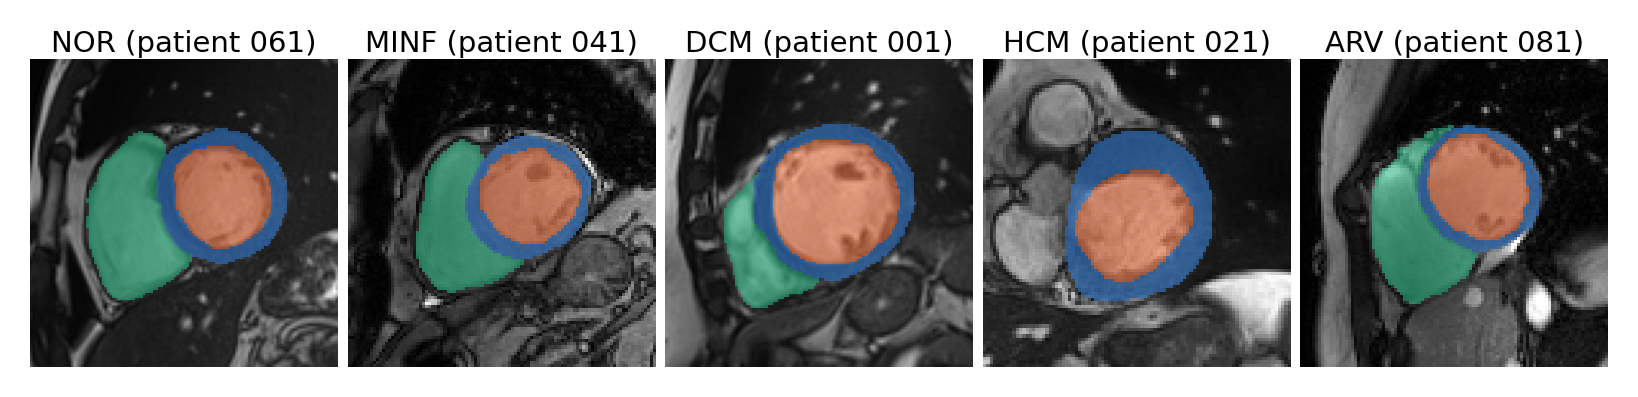
\includegraphics[width=\linewidth]{figs/data_overview.png}
  \caption{Mid-ventricular slice at end-diastole of the first training patient of each group, with the segmentation: RV (green), myocardium (blue), LV cavity (orange).}
  \label{fig:data}
\end{figure}

\paragraph{No data augmentation}
Geometric augmentation of the masks (rotations, translations, flips) is of no use for this task: all our features are measured in millimeters on the segmentations and are invariant to these transformations. A zoom that does not update the voxel spacing would change the volumes without changing the label, and would therefore add label noise. We do not augment the data.

\paragraph{Protocol}
All accuracies of this report are estimated by nested cross-validation \citep{varma2006}. The outer loop is a stratified 5-fold cross-validation, repeated 10 times with different shuffles; every patient receives one out-of-fold prediction per repeat. Inside each training fold, a stratified 5-fold cross-validation selects the hyper-parameters, and the feature scaling is fitted on the training fold only. We report the mean and standard deviation of the accuracy over repeats. Classes are balanced, so the balanced accuracy equals the accuracy; macro-F1 and per-class recalls are in Appendix~\ref{app:bench}. All configurations use the same outer splits, so we also report their paired difference with the best configuration. The standard deviation over repeats ignores the variability due to the sample itself \citep{nadeau2003}: with 100 patients, differences of one or two points should not be over-interpreted.

\paragraph{Implementation}
The code is a Python package and six scripts (indexing, LV reconstruction, features, protocol study, benchmark, final model), built on scikit-learn \citep{pedregosa2011}, PyTorch \citep{paszke2019}, SciPy, scikit-image and XGBoost \citep{chen2016}. Every run records its configuration, library versions, metrics, tables and figures (Appendix~\ref{app:runs}). Everything runs on an Apple M3 laptop in about 1 hour and 30 minutes, most of it spent training MLP ensembles inside the nested cross-validation.

\section{Method}
\label{sec:method}
\subsection{Reconstruction of the LV cavity}
\label{sec:lv-method}
In the test segmentations, the LV cavity is background enclosed by the myocardium. A natural reconstruction is to take, slice by slice, the holes of the myocardium mask (\emph{fill}). This fails on slices where the myocardial ring is open, typically the most basal one, where the myocardium does not fully surround the cavity: the slice then gets no cavity at all. We add a fallback (\emph{fill+hull}): on a slice with myocardium but no hole, the cavity is the convex hull of the myocardium minus the myocardium itself, restricted to background voxels. On apical slices, where the myocardium is a solid cap, this hull is a thin sliver; we keep it only if its area is at least 25\% of the myocardium area. Both methods are evaluated on the training set, where the true cavity is known, by removing it and reconstructing it (Section~\ref{sec:lv}).

\subsection{Features}
Table~\ref{tab:features} lists the features. The 21 \emph{volumetric} features are classical biomarkers: LV and RV volumes at ED and ES, ejection fractions, the myocardial mass (myocardium volume times 1.05 g/mL), volumes and mass indexed by the body surface area (BSA) computed with the Mosteller formula \citep{mosteller1987}, RV / LV ratios, height and weight.

None of them describes the shape of the myocardial wall, although wall thickness defines HCM \citep{elliott2014} and an infarct leaves a thin, akinetic segment \citep{thygesen2019}. We therefore add 11 \emph{thickness} features, in the spirit of the ACDC entries \citep{isensee2017,wolterink2017,khened2017}. On each slice that contains both myocardium and cavity, we compute the Euclidean distance transform (in mm) of the region formed by the myocardium and the cavity, and read it at every myocardium pixel that touches the cavity: this is the distance from the inner border of the wall to its outer border, i.e.\ the local wall thickness. For ED and ES, we summarize these samples by their mean and maximum, the largest per-slice mean, the mean of the per-slice standard deviations (how uneven the wall is within a slice) and the standard deviation of the per-slice means (how uneven it is along the axis). The systolic thickening is the ratio of the mean thicknesses at ES and ED. We compare three feature sets: the 21 volumetric features, the same plus the 11 thickness features, and a \emph{compact} set of 12 BSA-indexed and thickness features without raw height and weight.

\begin{table}[!htb]
\centering
\small
% Written by hand from final/cardiac/features.py (definitions in Appendix, tabs/supp/features_full.tex).
\begin{tabular}{p{0.2\linewidth}rp{0.62\linewidth}}
\toprule
Group & Count & Features\\
\midrule
LV & 6 & ED and ES volumes, ejection fraction, stroke volume, ED and ES volumes / BSA\\
RV & 5 & ED and ES volumes, ejection fraction, ED and ES volumes / BSA\\
Myocardium & 5 & mass (mean of ED and ES), mass / BSA, ES / ED mass, ED mass / LV ED volume, mean mass / LV ED volume\\
RV / LV & 2 & volume ratios at ED and at ES\\
Patient & 3 & height, weight, body surface area (Mosteller)\\
\midrule
Wall thickness & 11 & at ED and at ES: mean, maximum, largest per-slice mean, mean of per-slice standard deviations, standard deviation of per-slice means; systolic thickening (ES / ED mean thickness)\\
\bottomrule
\end{tabular}
\caption{Features. The first 21 are the \emph{volumetric} features. The \emph{compact} set keeps 12 of them: the 6 indexed volumes and ejection fractions, mass / BSA, the RV / LV volume ratio at ED, mean mass / LV ED volume, the largest per-slice mean and the mean per-slice standard deviation of the ED wall thickness, and the systolic thickening.}
\label{tab:features}

\end{table}

\subsection{Classifiers}
Every model is a pipeline that standardizes the features on the training data. We compare logistic regression, linear and RBF SVMs, $k$ nearest neighbors, random forests, extremely randomized trees and XGBoost, with the hyper-parameter grids of Appendix~\ref{app:bench}, selected by the inner cross-validation.

\paragraph{MLP ensemble}
We use an ensemble of 50 MLPs with 4 hidden layers of 32 units, batch normalization and leaky ReLUs, each trained on a random 75\% of the training patients and a random two thirds of the features, for 200 epochs with Adam (learning rate $10^{-3}$, batches of 30). The ensemble averages their class probabilities. We train the 50 networks as one batched network: the weights of each layer are stacked into a tensor, each network sees its own patients and batch-normalization statistics, and dropped features are set to zero, which is equivalent to removing them. This gives the same result as 50 separate networks about 50 times faster, which makes nested cross-validation affordable.

\paragraph{Soft vote}
The MLP ensemble is combined with a random forest or a linear SVM by averaging their probabilities with a weight $\alpha$ on the MLP:
\begin{equation}
  p(y\mid x) = \alpha\, p_{\mathrm{MLP}}(y\mid x) + (1-\alpha)\, p_{\mathrm{other}}(y\mid x).
  \label{eq:softvote}
\end{equation}
We choose $\alpha\in\{0, 0.1, \dots, 1\}$ inside each training fold, from the out-of-fold probabilities of an inner 5-fold cross-validation, breaking ties towards $\alpha=0.5$; the two models are then refitted on the whole training fold. The SVM probabilities come from Platt scaling \citep{platt1999}.

\section{Experiments}

\subsection{Single-split model selection is optimistic}
\label{sec:protocol-study}
A common way to tune classifiers on a small dataset is to standardize the features of all patients, draw one stratified 5-fold split, score every configuration of a grid on it, and report the best score. We applied this protocol to standard classifiers on the 21 volumetric features (true LV), with grids of 12 to 135 configurations, and compared it with nested cross-validation on the same grids (Table~\ref{tab:protocol-study}).

% Generated by regenerate_figures.py from final/results/protocol_study
\begin{table}[!htb]
\centering
\small
\setlength{\tabcolsep}{4pt}
\begin{adjustbox}{max width=\linewidth}
\begin{tabular}{lrrrrr}
\toprule
& \multicolumn{4}{c}{Single split (scaler fitted on all patients)} & \\
\cmidrule(lr){2-5}
Model & Configs & Tied best & Median & Best & Nested CV\\
\midrule
Random forest & 30 & 12 & 0.930 & 0.940 & 0.930 $\pm$ 0.012\\
XGBoost & 135 & 97 & 0.910 & 0.910 & 0.910 $\pm$ 0.007\\
SVM (linear or RBF) & 12 & 2 & 0.925 & 0.950 & 0.936 $\pm$ 0.009\\
$k$-NN & 16 & 3 & 0.880 & 0.930 & 0.904 $\pm$ 0.021\\
MLP ensemble & -- & -- & -- & 0.936 & 0.926 $\pm$ 0.011\\
MLP + RF & 11 & -- & -- & 0.938 & 0.926 $\pm$ 0.005\\
MLP + linear SVM & 11 & -- & -- & 0.938 & 0.932 $\pm$ 0.008\\
\bottomrule
\end{tabular}
\end{adjustbox}
\caption{Model selection on a single split vs nested cross-validation (21 volumetric features, true LV).
\emph{Single split}: every configuration of the grid scored on one stratified 5-fold split; \emph{Best}: the best
of them, \emph{Tied best}: number of configurations reaching it, \emph{Median}: median over the grid. For the
MLP ensemble (no grid), mean over 5 seeds; for the soft votes, best $\alpha$ on the split, mean over 5 seeds.
\emph{Nested CV}: same grids, selected inside the training folds, mean $\pm$ std over 5 repeats.}
\label{tab:protocol-study}
\end{table}


On the single split, the best configurations reach 0.91 to 0.95, but the grids barely discriminate between configurations: for the random forest, 12 of the 30 configurations tie at the best score; for XGBoost, 97 of 135 do. Reporting the best of the grid is reporting the luckiest configuration on one split. Under nested cross-validation, with the same grids selected inside the training folds and 5 repeated splits, every model loses between 0 and 2.6 points: the SVM drops from 0.95 to $0.936 \pm 0.009$, $k$-NN from 0.93 to $0.904 \pm 0.021$, the random forest from 0.94 to $0.930 \pm 0.012$. XGBoost does not change, because almost all its configurations score the same. On the volumetric features, the seven models end up within about 3 points of each other (0.904 to 0.936), and no model is clearly better than the others.

Three other shortcuts matter for the ensembles (Figure~\ref{fig:protocol-study}). First, scoring MLPs on the patients they were trained on cannot select hyper-parameters: every configuration we tried reaches 100\%, against 92 to 93\% in cross-validation (Appendix~\ref{app:protocol}). Second, choosing the weight $\alpha$ of the soft vote (Eq.~\ref{eq:softvote}) on the evaluation folds selects noise: with five random seeds of the MLP ensemble, the best $\alpha$ on the same split is 0.0, 0.9, 0.2, 0.9 and 0.8 for MLP + RF, and 0.1, 0.4, 0.9, 0.5 and 0.3 for MLP + SVM, and on every curve all values of $\alpha$ fall within 3 patients of each other. Third, selecting the 16 most important features on all patients before the cross-validation leaks the evaluation folds, but the effect is negligible here (0.924 against 0.923 when selected inside the folds; Appendix~\ref{app:protocol}). All the following results therefore use nested cross-validation, with $\alpha$ chosen inside the training folds.

\begin{figure}[!htb]
  \centering
  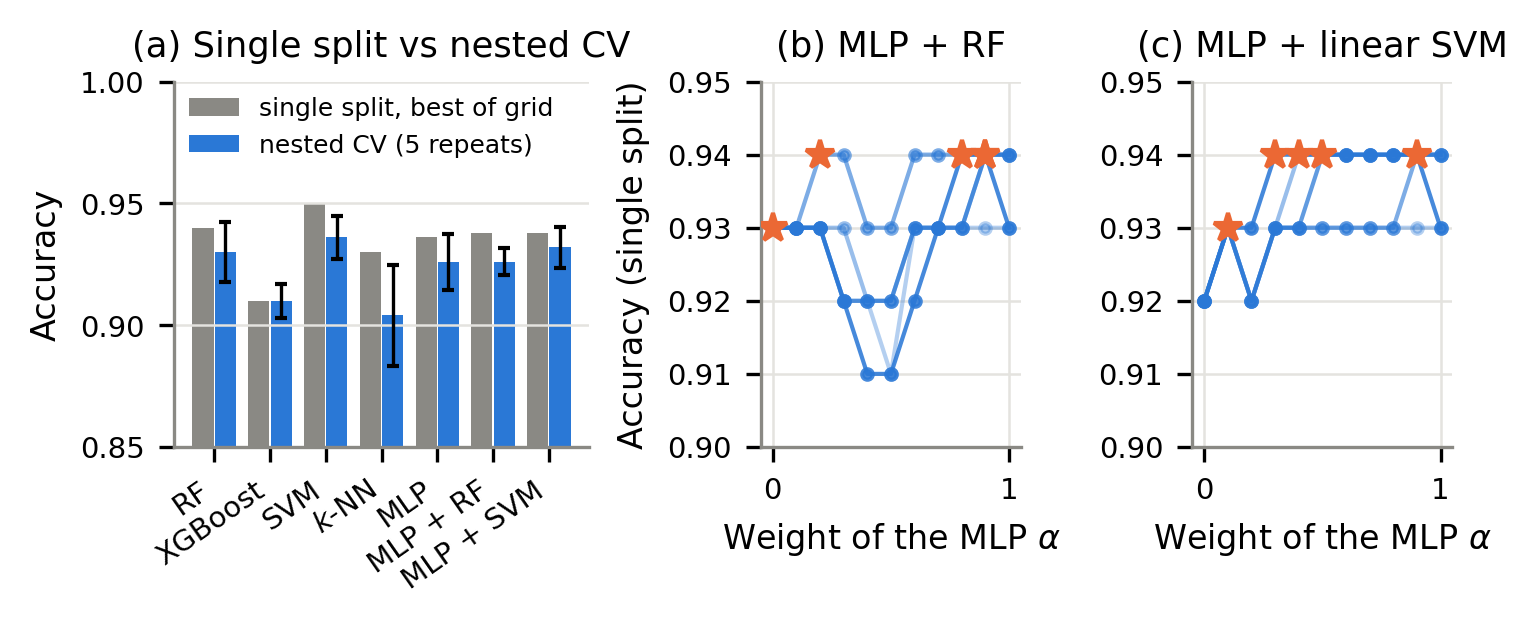
\includegraphics[width=\linewidth]{figs/protocol.png}
  \caption{(a) Best single-split accuracy and nested-CV accuracy (mean $\pm$ std over 5 repeats) of the same models and grids (21 volumetric features). (b, c) Accuracy of the soft vote (Eq.~\ref{eq:softvote}) on a single split as a function of $\alpha$, for five random seeds of the MLP ensemble (one curve each); stars mark the best $\alpha$ of each curve.}
  \label{fig:protocol-study}
\end{figure}

\subsection{Reconstruction of the LV cavity}
\label{sec:lv}
Filling the holes of the myocardium recovers the true cavity almost perfectly: 193 of the 200 training volumes are reconstructed voxel for voxel, and the mean Dice coefficient \citep{dice1945} is 0.997 (Table~\ref{tab:lv}). The 7 other volumes each miss one slice, the most basal one, where the myocardium is open (Figure~\ref{fig:lv}a, b). The volume error then reaches 29 mL and the ejection-fraction error 12.8 points, enough to move a patient across a diagnostic threshold. The convex-hull fallback recovers all 7 slices (minimum Dice 0.990, maximum ejection-fraction error 0.8 points). Without the area threshold, it also creates 20 spurious slices on apical caps; with a threshold of 25\% or 50\% of the myocardium area, it creates none. On the test set, the fallback never triggers: all test slices with myocardium are either closed rings or caps, so both methods give exactly the same test cavities.

% Generated by regenerate_figures.py from final/results/lv_reconstruction/tables/summary.csv
\begin{table}[!htb]
\centering
\small
\setlength{\tabcolsep}{4pt}
\begin{adjustbox}{max width=\linewidth}
\begin{tabular}{lrrrrrrrr}
\toprule
& \multicolumn{2}{c}{Dice} & Exact & Max $|\Delta V|$ & \multicolumn{2}{c}{Slices} & \multicolumn{2}{c}{$|\Delta$EF$|$ (points)}\\
\cmidrule(lr){2-3}\cmidrule(lr){6-7}\cmidrule(lr){8-9}
Method & mean & min & volumes & (mL) & missed & spurious & mean & max\\
\midrule
Filling (holes of the myocardium) & 0.9969 & 0.832 & 193 & 28.7 & 7 & 0 & 0.57 & 12.8\\
+ convex hull, no threshold & 0.9995 & 0.988 & 175 & 3.1 & 0 & 20 & 0.07 & 0.8\\
+ convex hull, area $\geq$ 25\% (ours) & 0.9998 & 0.990 & 193 & 3.1 & 0 & 0 & 0.03 & 0.8\\
+ convex hull, area $\geq$ 50\% & 0.9998 & 0.990 & 193 & 3.1 & 0 & 0 & 0.03 & 0.8\\
\bottomrule
\end{tabular}
\end{adjustbox}
\caption{Reconstruction of the LV cavity on the 200 training volumes (100 patients, ED and ES), compared with the
true LV. \emph{Exact}: volumes reconstructed voxel for voxel. EF errors are per patient.}
\label{tab:lv}
\end{table}


\begin{figure}[!htb]
  \centering
  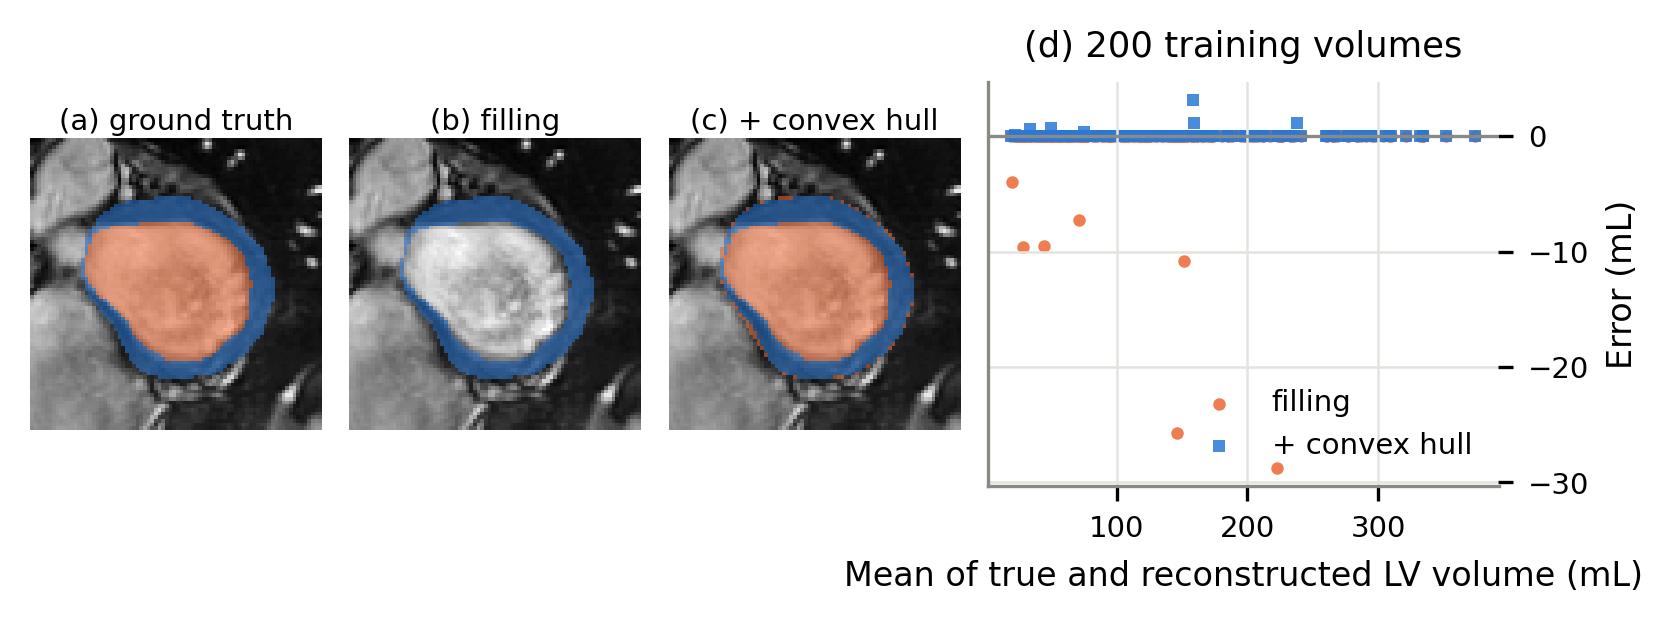
\includegraphics[width=\linewidth]{figs/lv_reconstruction.png}
  \caption{(a--c) Basal slice of training patient 011 at ED, whose myocardium does not close around the cavity: true cavity, filling (no cavity on this slice) and convex-hull fallback. (d) Error of the reconstructed LV volume against the mean of the true and reconstructed volumes \citep{blandaltman1986}, for the 200 training volumes.}
  \label{fig:lv}
\end{figure}

\subsection{Consistency of training and test features}
\label{sec:protocol}
A natural approach is to train the classifiers on features computed with the true LV, available for the training patients, and to apply them to test features computed with a reconstructed LV. To measure the effect of this mismatch, we train on one LV source and evaluate on another, for the same training patients (Table~\ref{tab:protocol}). The differences between protocols are at most 1.6 points and have no consistent sign: the linear SVM on 32 features scores 0.954, 0.956, 0.959 and 0.956 under the four protocols. Only 7 of the 100 training patients have features that differ at all between the true and reconstructed LV (Appendix~\ref{app:lv}); the largest changes, up to 98\% of the ejection fraction of one patient, occur with the filling without fallback. This mismatch is therefore harmless on this data. We nevertheless train and evaluate with \emph{fill+hull}, the same reconstruction as for the test patients.

% Generated by regenerate_figures.py from final/results/lv_protocol/tables/summary_mean.csv
\begin{table}[!htb]
\centering
\small
\setlength{\tabcolsep}{4pt}
\begin{adjustbox}{max width=\linewidth}
\begin{tabular}{lcccc}
\toprule
LV of training $\to$ evaluated patients & true $\to$ true & true $\to$ fill & fill $\to$ fill & fill+hull $\to$ fill+hull\\
\midrule
\multicolumn{5}{l}{\emph{Volumetric (21)}}\\
\quad Logistic regression & 0.897 $\pm$ 0.018 & 0.900 $\pm$ 0.014 & 0.900 $\pm$ 0.016 & 0.896 $\pm$ 0.016\\
\quad Linear SVM & 0.928 $\pm$ 0.014 & 0.928 $\pm$ 0.015 & 0.925 $\pm$ 0.014 & 0.925 $\pm$ 0.016\\
\quad Random forest & 0.922 $\pm$ 0.014 & 0.929 $\pm$ 0.015 & 0.932 $\pm$ 0.014 & 0.923 $\pm$ 0.016\\
\quad XGBoost & 0.918 $\pm$ 0.015 & 0.927 $\pm$ 0.013 & 0.928 $\pm$ 0.013 & 0.920 $\pm$ 0.013\\
\multicolumn{5}{l}{\emph{Volumetric + thickness (32)}}\\
\quad Logistic regression & 0.943 $\pm$ 0.014 & 0.937 $\pm$ 0.012 & 0.937 $\pm$ 0.012 & 0.953 $\pm$ 0.014\\
\quad Linear SVM & 0.954 $\pm$ 0.013 & 0.956 $\pm$ 0.013 & 0.959 $\pm$ 0.007 & 0.956 $\pm$ 0.014\\
\quad Random forest & 0.938 $\pm$ 0.012 & 0.944 $\pm$ 0.012 & 0.941 $\pm$ 0.014 & 0.938 $\pm$ 0.015\\
\quad XGBoost & 0.915 $\pm$ 0.020 & 0.922 $\pm$ 0.019 & 0.928 $\pm$ 0.020 & 0.916 $\pm$ 0.021\\
\bottomrule
\end{tabular}
\end{adjustbox}
\caption{Effect of the LV used to compute the features (nested CV, 10 repeats). \emph{true}: ground-truth LV
(training set only); \emph{fill}: filling; \emph{fill+hull}: filling with the convex-hull fallback.
``true $\to$ fill'' is the situation of a model trained with the true LV and applied to the test set.}
\label{tab:protocol}
\end{table}


\subsection{Comparison of features and classifiers}
\label{sec:bench}
Table~\ref{tab:benchmark} and Figure~\ref{fig:bench} compare 10 classifiers on the three feature sets. On the 21 volumetric features, accuracies range from 0.895 ($k$-NN) to 0.931 (extra trees), and the ensembles do not beat their components. Adding the 11 thickness features improves most models: logistic regression by 5.7 points, the MLP ensemble by 3.7, the linear SVM by 3.1 and MLP + linear SVM by 3.9. The trees gain little (random forest +1.5, extra trees +0.6) and XGBoost does not gain at all. The best configuration is MLP + linear SVM on the 32 features, with $0.966 \pm 0.011$. Its paired advantage over the MLP ensemble alone is $0.009 \pm 0.008$, and over the linear SVM alone $0.010 \pm 0.009$, i.e.\ one patient on average. The compact set (12 features) reaches 0.955 with the same ensemble. It gives the best HCM recall (1.00 for logistic regression and the RBF SVM), but loses MINF patients (recall 0.89 to 0.91 for the linear models, SVMs and MLP ensembles, against 0.95 to 0.96 with 32 features; Appendix~\ref{app:bench}).

% Generated by regenerate_figures.py from final/results/benchmark/tables/summary_mean.csv
\begin{table}[!htb]
\centering
\small
\setlength{\tabcolsep}{5pt}
\begin{tabular}{lccc}
\toprule
Model & Volumetric (21) & Volumetric + thickness (32) & Compact (12)\\
\midrule
Logistic regression & 0.896 $\pm$ 0.016 & 0.953 $\pm$ 0.014 & 0.942 $\pm$ 0.015\\
Linear SVM & 0.925 $\pm$ 0.016 & 0.956 $\pm$ 0.014 & 0.927 $\pm$ 0.009\\
RBF SVM & 0.923 $\pm$ 0.022 & 0.945 $\pm$ 0.012 & 0.944 $\pm$ 0.019\\
$k$-NN & 0.895 $\pm$ 0.010 & 0.902 $\pm$ 0.023 & 0.932 $\pm$ 0.012\\
\midrule
Random forest & 0.923 $\pm$ 0.016 & 0.938 $\pm$ 0.015 & 0.925 $\pm$ 0.019\\
Extra trees & \textbf{0.931} $\pm$ 0.010 & 0.937 $\pm$ 0.012 & 0.940 $\pm$ 0.009\\
XGBoost & 0.920 $\pm$ 0.013 & 0.916 $\pm$ 0.021 & 0.915 $\pm$ 0.022\\
\midrule
MLP ensemble & 0.920 $\pm$ 0.012 & 0.957 $\pm$ 0.008 & 0.953 $\pm$ 0.014\\
MLP + RF & 0.925 $\pm$ 0.012 & 0.954 $\pm$ 0.010 & 0.952 $\pm$ 0.019\\
MLP + linear SVM & 0.927 $\pm$ 0.012 & \textbf{0.966} $\pm$ 0.011 & \textbf{0.955} $\pm$ 0.008\\
\bottomrule
\end{tabular}
\caption{Nested-CV accuracy (mean $\pm$ std over 10 repeats of stratified 5-fold CV) with the LV reconstructed in
training and evaluated patients, as for the test set. Hyper-parameters and the ensemble weight $\alpha$ are
selected by an inner 5-fold CV. Best value of each column in bold. Classes are balanced, so the balanced accuracy
equals the accuracy.}
\label{tab:benchmark}
\end{table}


\begin{figure}[!htb]
  \centering
  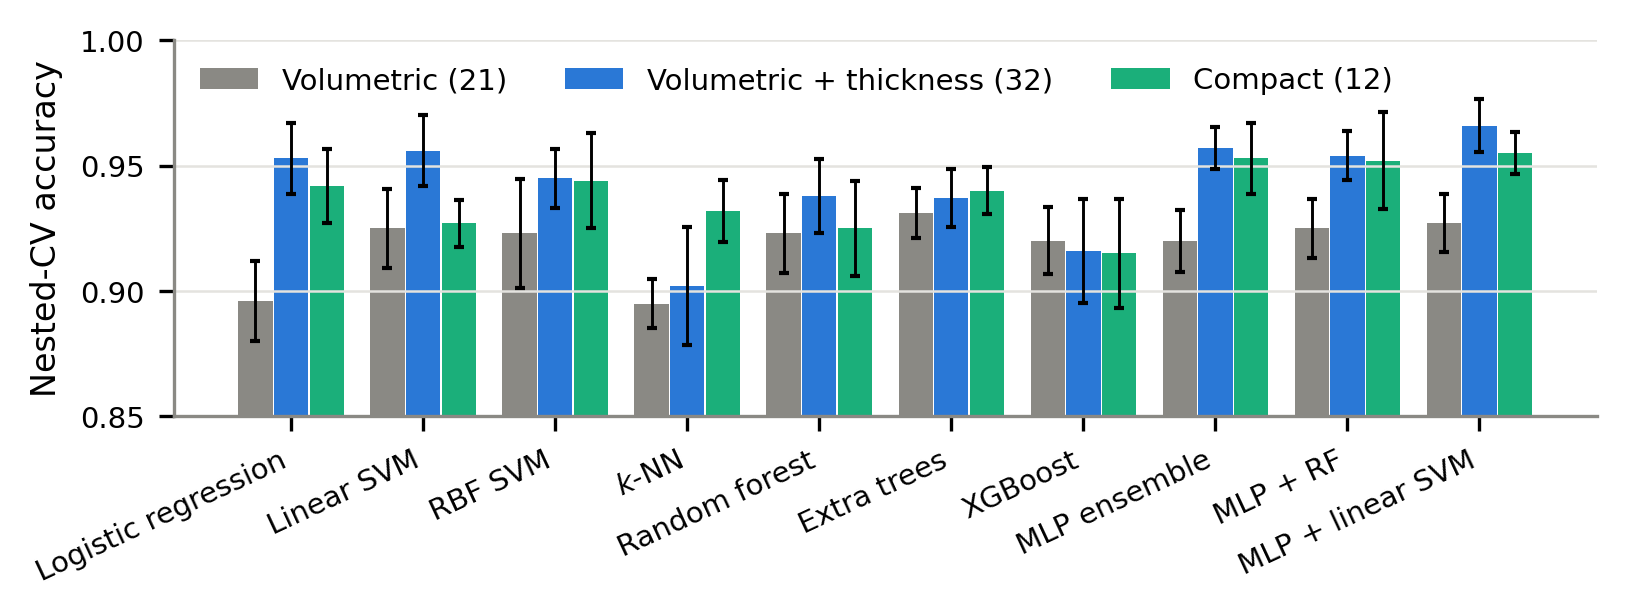
\includegraphics[width=\linewidth]{figs/benchmark.png}
  \caption{Nested-CV accuracy of each classifier on the three feature sets (mean $\pm$ std over 10 repeats).}
  \label{fig:bench}
\end{figure}

Figure~\ref{fig:features} shows why the thickness features help. The LV ejection fraction and indexed volume separate the groups with a dilated, poorly contracting LV (MINF and DCM) from the others, and the RV ejection fraction isolates ARV and part of DCM. The myocardial mass separates HCM and DCM from the others, but not from each other. The thickest slice at ED isolates HCM. The variability of the wall thickness within a slice at ES is high for HCM and MINF and low for DCM: an infarct thins one segment of the wall and leaves the others thick, while a dilated cardiomyopathy thins the whole wall evenly. This feature thus separates MINF from DCM, the pair that the volumes confuse most.

\begin{figure}[!htb]
  \centering
  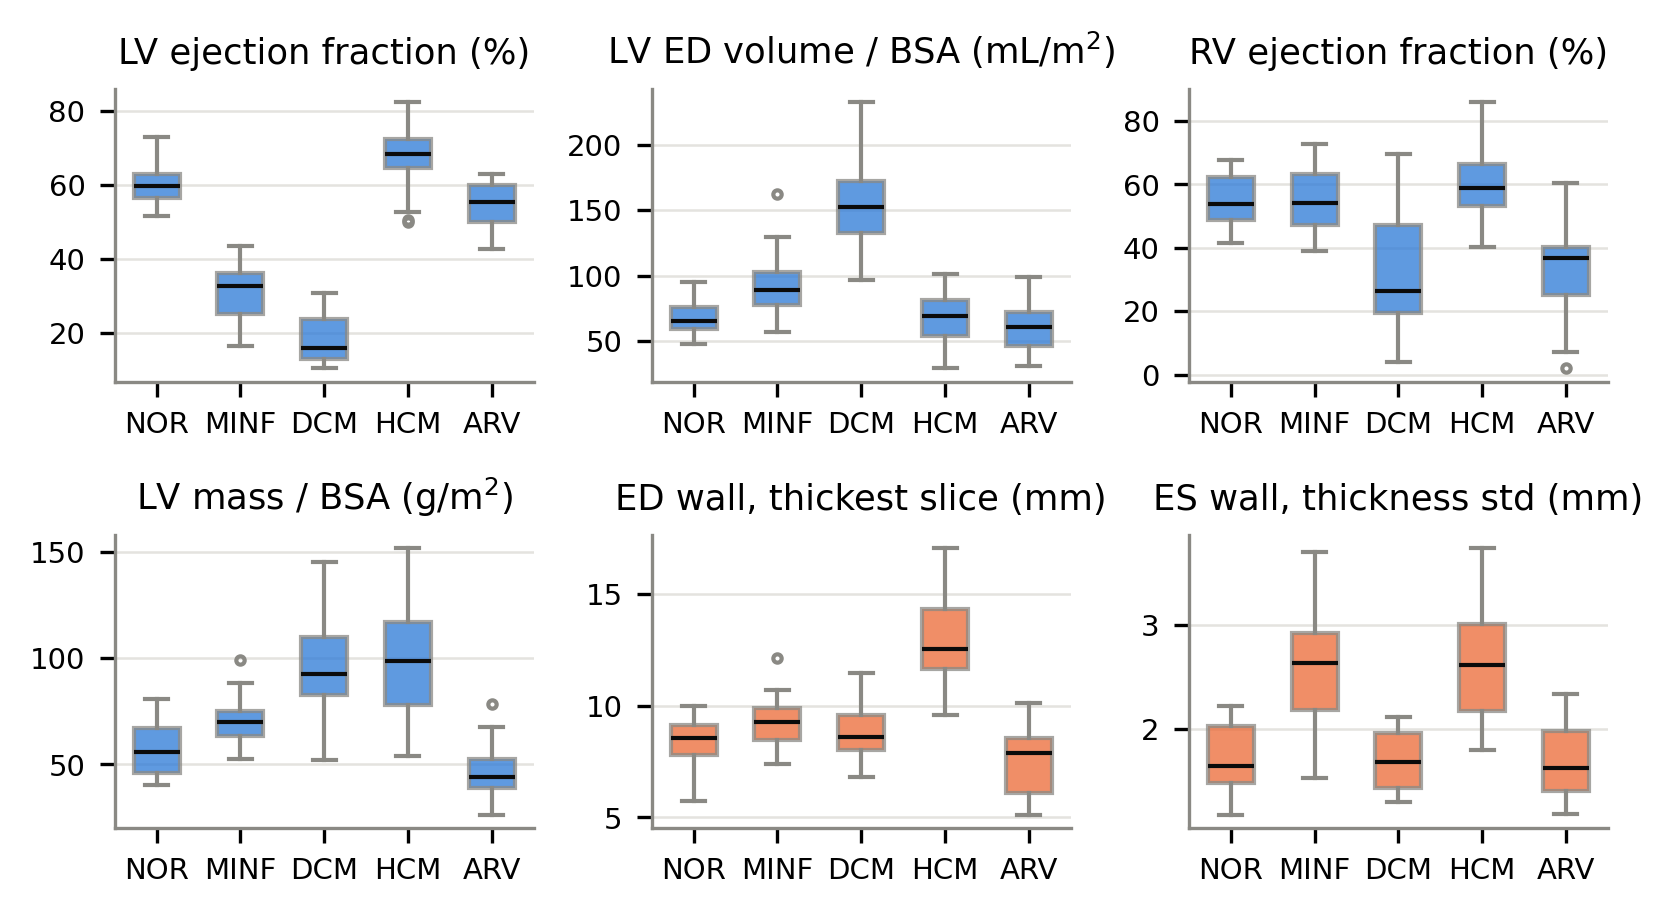
\includegraphics[width=\linewidth]{figs/features_by_class.png}
  \caption{Distribution of six features per group (100 training patients, reconstructed LV). Blue: volumetric features; orange: thickness features. Boxes: quartiles; whiskers: 1.5 times the interquartile range.}
  \label{fig:features}
\end{figure}

\subsection{Final model}
\label{sec:final}
The final model is the soft vote of the MLP ensemble and a linear SVM ($C=1$) on the 32 features, with the LV reconstructed by \emph{fill+hull}. The inner cross-validation selects $\alpha=0.5$ in 33 of the 50 outer folds and on the whole training set. Its nested-CV accuracy is $0.966 \pm 0.011$ (0.94 to 0.98 over the repeats), with recalls between 0.945 (DCM) and 0.985 (NOR) (Figure~\ref{fig:final}a; Appendix~\ref{app:final}).

\paragraph{Errors}
Over the 10 repeats, 9 patients are misclassified at least once, and only 3 more than twice. MINF patient 050 is always predicted DCM: its LV ejection fraction is 16\% and its indexed ED volume 163 mL/m$^2$, the values of a typical DCM. DCM patient 002 is predicted MINF in 9 repeats out of 10, with an unusually uneven wall for a DCM. HCM patient 022 is predicted NOR in 4 repeats and MINF in 1; its ejection fraction (65\%) and wall thickness lie between those of the NOR and HCM groups. The MINF / DCM confusion is clinically expected: an extensive infarct can dilate the LV until it resembles a dilated cardiomyopathy, and conversely, and the two are told apart by the localization of the lesion (late gadolinium enhancement), which segmentations do not show.

\paragraph{Feature importance}
Permuting the within-slice variability of the ES wall thickness costs 5 points of held-out accuracy, twice as much as any other feature (Figure~\ref{fig:final}b). The LV and RV ejection fractions, the stroke volume and the RV volume at ES follow. Many features are strongly correlated (volumes and their indexed versions, the two mass / volume ratios), so the importance of each is shared with its correlates \citep{strobl2007}, and the standard deviations are large.

\begin{figure}[!htb]
  \centering
  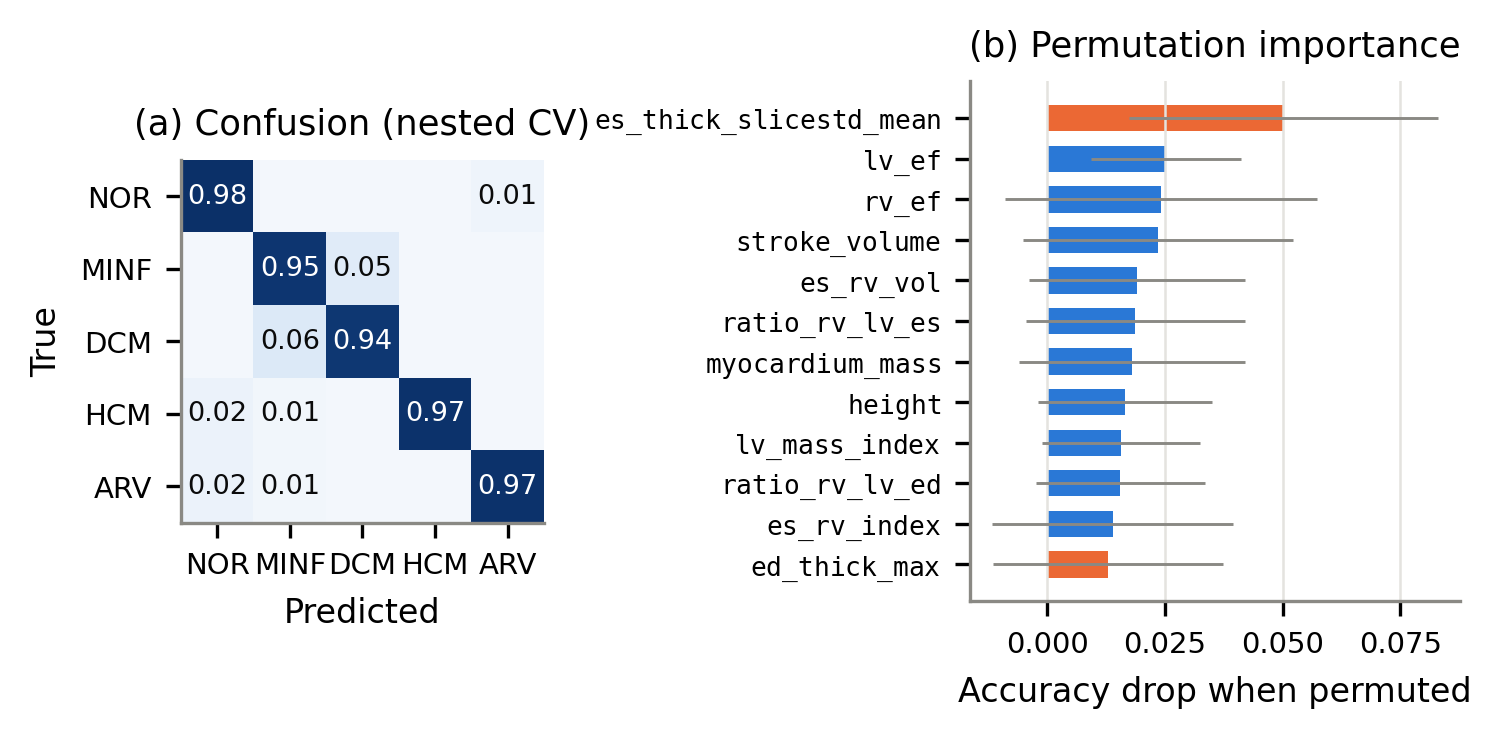
\includegraphics[width=\linewidth]{figs/final_model.png}
  \caption{Final model. (a) Confusion matrix pooled over the 10 repeats of the nested cross-validation (rows sum to 1). (b) Permutation importance of the 12 most important features on held-out folds (mean $\pm$ std over 15 folds); orange: thickness features.}
  \label{fig:final}
\end{figure}

\paragraph{Test predictions}
Fitted on the 100 training patients, the model predicts 12 NOR, 8 MINF, 11 DCM, 9 HCM and 10 ARV patients among the 50 test patients, close to the 10 per group of the ACDC test set. The mean probability of the predicted class is 0.81, and 6 patients have a probability below 0.6. These predictions cannot be scored here: the test labels are hidden behind the course leaderboard (Appendix~\ref{app:final}).

\section{Discussion}
\paragraph{Information matters more than the classifier}
On 100 patients, selecting among dozens of nearly tied configurations on a single split and reporting the best score adds one to three points of accuracy, about the size of the differences one would use to choose between models or ensemble weights. Under a protocol that removes this bias, changing the classifier, combining several or tuning their weights moves the accuracy by at most a few patients, whereas adding wall-thickness features moves it by 3 to 6 points. With clinically defined groups, the information given to the classifier matters more than the classifier. Several possible sources of bias turned out to be harmless on this data: training on the true LV and testing on a reconstructed one, or selecting features before the cross-validation. They still had to be measured, because each of them could matter on another dataset.

\paragraph{Why the ensembles help only with good features}
On the 21 volumetric features, the MLP ensemble, the SVM and their average all reach about 0.92 to 0.93. Their errors are then largely shared, which leaves little for averaging to correct. With the thickness features, the MLP ensemble and the linear SVM both reach about 0.956, and their average 0.966. The gain of one patient on average is within the noise of our protocol, but it has a consistent sign: on the same splits, the average is better than the linear SVM in 7 repeats out of 10 and than the MLP ensemble in 6, and never worse than either. A linear SVM alone would be an equally defensible choice, and a simpler one to explain.

\paragraph{Comparison with ACDC}
The best ACDC entries reported 92 to 96\% accuracy on the 50 test patients, with features computed on their own automatic segmentations \citep{bernard2018,isensee2017,khened2017}. Our 96.6\% is a cross-validated estimate on the 100 training patients with ground-truth segmentations (and an almost exact reconstruction of the LV), so it is not directly comparable: errors of an automatic segmentation would propagate to the features, and our protocol shares the same 100 patients between model selection and evaluation, even if never within one fold. \citet{isensee2017} also used the whole cardiac cycle, not only ED and ES, which describes the motion of the wall directly.

\paragraph{Limitations}
The test labels are not available to us, so our test predictions cannot be scored, and all our accuracies are estimated on 100 patients. The standard deviations over repeats measure the variability due to the splits, not the variability due to the patients \citep{nadeau2003}; a confidence interval for a new sample of patients would be wider. The choice of the final model among 30 configurations of the benchmark is itself a selection on the same data, which makes its $0.966$ slightly optimistic; the difference with the next configurations is about one patient. The feature sets and the thickness descriptors were designed with the training data in view, without a separate validation set. Finally, the MINF / DCM confusion cannot be resolved by segmentations of two frames: it would require the localization of the lesion or the motion of each wall segment.

\section{Conclusion}
We classified cardiac pathologies from ED and ES segmentations, separating strictly the data used to select models from the data used to score them. On 21 volumetric biomarkers, selecting hyper-parameters on a single split gives accuracies of 0.91 to 0.95, whereas nested cross-validation gives 0.90 to 0.94 for the same models, none of which stands out; ensemble weights chosen on the evaluation folds are noise. The missing LV cavity of the test patients is recovered almost exactly by filling the myocardium, and a convex-hull fallback fixes the open basal slices; whether training uses the true or the reconstructed cavity makes no measurable difference. The step that improves classification is describing the myocardial wall: thickness features raise the accuracy by 3 to 6 points, and an average of an MLP ensemble and a linear SVM reaches $0.966 \pm 0.011$. Its remaining errors are infarcted hearts that look dilated and the converse. Future work should evaluate the pipeline on automatic segmentations of the test images, add features of the whole cardiac cycle such as regional wall motion, and score the predictions on held-out labels.


\section*{Reproducibility Statement}
All results are produced by six scripts from the segmentations and the metadata, with fixed seeds; each run records its configuration, library versions, metrics, tables and figures. The data folders are only read: any LV label found in a test segmentation is ignored when it is loaded. Appendix~\ref{app:features} defines every feature, Appendix~\ref{app:bench} lists the hyper-parameter grids and Appendix~\ref{app:runs} lists the experiments, their running times and the library versions. All figures and tables of this report are regenerated from the experiment outputs by two scripts.

\section*{AI Use Statement}
Generative AI tools were used to generate portions of the project code and to assist with drafting and editing this report. The author reviewed and verified the AI-generated code and results. The project's ideas and research questions were developed by the author and were not generated by AI.


\bibliography{references}
\bibliographystyle{iclr2025_conference}

\clearpage
\appendix
% Appendix. Figures in figs/supp/ and tables in tabs/supp/ are generated by regenerate_supplementary.py
% from final/results; rerun it after rerunning the experiments. Floats use [H] so that every figure
% and table stays in its subsection.

\begin{center}
  {\LARGE\bfseries Appendix}
\end{center}

All figures and tables of this appendix are produced from the outputs of the experiment scripts. Unless stated otherwise, accuracies are nested-CV means $\pm$ standard deviations over 10 repeats of stratified 5-fold cross-validation, with the LV reconstructed by \emph{fill+hull} for training and evaluated patients.

\startcontents[appendix]
\printcontents[appendix]{}{1}{\setcounter{tocdepth}{2}\section*{Contents}\footnotesize}

\clearpage
% ==========================================================================================
\section{Dataset}
\label{app:data}

\subsection{Patients}
Table~\ref{tab:supp-classes} describes the patients. ARV patients are lighter on average and have more slices, with a smaller slice step; the test set has more slices on average than the training set. All our features are computed in millimeters, so they do not depend on the resolution, but the thickness features are sampled more coarsely along the long axis when the slice step is large.

% Generated by regenerate_supplementary.py from results/dataset/tables/class_stats.csv
\begin{table}[H]
\centering
\small
\setlength{\tabcolsep}{4pt}
\begin{adjustbox}{max width=\linewidth}
\begin{tabular}{lrrrrrr}
\toprule
Group & Patients & Height (cm) & Weight (kg) & Slices & In-plane (mm) & Slice step (mm) \\
\midrule
DCM & 20 & 171.1 & 75.5 & 9.8 & 1.51 & 10.0 \\
HCM & 20 & 169.8 & 80.3 & 9.4 & 1.49 & 9.8 \\
MINF & 20 & 172.2 & 74.2 & 8.7 & 1.49 & 9.8 \\
NOR & 20 & 172.2 & 77.9 & 8.5 & 1.52 & 9.8 \\
ARV & 20 & 168.9 & 66.9 & 11.2 & 1.55 & 7.3 \\
Test (n=50) & 50 & 170.0 & 80.7 & 10.8 & 1.52 & 9.1 \\
\bottomrule
\end{tabular}
\end{adjustbox}
\caption{Patients per class (means). The training set has 20 patients per class; the test set has the same number of patients per class in ACDC, but its labels are not available. Slice counts range from 6 to 21; slice steps take the values 5, 6.5, 7, 10 mm.}
\label{tab:supp-classes}
\end{table}


\clearpage
% ==========================================================================================
\section{Features}
\label{app:features}

\subsection{Definitions and class means}
Table~\ref{tab:supp-features} defines the 32 features and gives their mean per group. Volumes are counted in voxels and multiplied by the voxel volume given in the file header. Wall-thickness samples are read on the Euclidean distance transform of the union of the myocardium and the cavity (filled), at the myocardium pixels that are 4-connected to the cavity, with the in-plane pixel spacing as sampling; slices without myocardium or without cavity are skipped.

% Generated by regenerate_supplementary.py from final/cache/features/train_fill_hull.csv
\begin{table}[H]
\centering
\scriptsize
\setlength{\tabcolsep}{4pt}
\begin{adjustbox}{max width=\linewidth}
\begin{tabular}{lp{0.4\linewidth}crrrrr}
\toprule
Feature & Definition & Set & NOR & MINF & DCM & HCM & ARV \\
\midrule
\texttt{ed\_lv\_vol} & LV volume at ED (mL) & V & 130.1 & 172.2 & 284.6 & 129.3 & 107.1 \\
\texttt{es\_lv\_vol} & LV volume at ES (mL) & V & 51.7 & 119.4 & 233.1 & 42.2 & 49.1 \\
\texttt{lv\_ef} & LV ejection fraction, $100\,(V_{ED}-V_{ES})/V_{ED}$ (\%) & V, C & 60.3 & 31.0 & 18.5 & 67.4 & 54.7 \\
\texttt{ed\_rv\_vol} & RV volume at ED (mL) & V & 153.2 & 119.1 & 178.0 & 118.3 & 196.3 \\
\texttt{es\_rv\_vol} & RV volume at ES (mL) & V & 68.8 & 54.7 & 125.6 & 46.1 & 134.1 \\
\texttt{rv\_ef} & RV ejection fraction (\%) & V, C & 55.1 & 55.5 & 31.8 & 59.8 & 31.4 \\
\texttt{myocardium\_mass} & Myocardial mass, $1.05$ g/mL $\times$ volume, mean of ED and ES (g) & V & 111.0 & 131.5 & 176.9 & 191.3 & 82.7 \\
\texttt{lv\_mass\_index} & Myocardial mass / BSA (g/m$^2$) & V, C & 57.6 & 70.3 & 95.8 & 99.4 & 46.5 \\
\texttt{stroke\_volume} & LV stroke volume, $V_{ED}-V_{ES}$ (mL) & V & 78.4 & 52.8 & 51.5 & 87.1 & 58.0 \\
\texttt{es\_lv\_index} & LV ES volume / BSA & V, C & 26.9 & 64.1 & 125.6 & 22.0 & 27.6 \\
\texttt{ed\_rv\_index} & RV ED volume / BSA & V, C & 79.6 & 63.3 & 94.2 & 60.9 & 111.9 \\
\texttt{ratio\_rv\_lv\_es} & RV / LV volume at ES & V & 1.33 & 0.49 & 0.53 & 1.17 & 3.16 \\
\texttt{ratio\_rv\_lv\_ed} & RV / LV volume at ED & V, C & 1.17 & 0.72 & 0.62 & 0.93 & 2.00 \\
\texttt{weight} & Weight (kg) & V & 77.9 & 74.2 & 75.5 & 80.3 & 66.9 \\
\texttt{height} & Height (cm) & V & 172.2 & 172.2 & 171.1 & 169.8 & 168.9 \\
\texttt{bsa} & Body surface area, Mosteller (m$^2$) & V & 1.92 & 1.88 & 1.88 & 1.94 & 1.76 \\
\texttt{ed\_lv\_index} & LV ED volume / BSA & V, C & 67.8 & 92.4 & 153.4 & 67.3 & 60.2 \\
\texttt{es\_rv\_index} & RV ES volume / BSA & V, C & 35.6 & 29.0 & 66.3 & 24.0 & 76.5 \\
\texttt{myocardium\_to\_lv\_ed} & ED myocardial mass / LV ED volume & V & 0.79 & 0.74 & 0.60 & 1.40 & 0.75 \\
\texttt{mass\_to\_edv\_ratio} & Mean myocardial mass / LV ED volume & V, C & 0.86 & 0.79 & 0.63 & 1.51 & 0.80 \\
\texttt{mass\_ratio\_systole\_diastole} & ES / ED myocardial mass & V & 1.17 & 1.14 & 1.08 & 1.18 & 1.15 \\
\texttt{ed\_thick\_mean} & ED wall thickness, mean over all samples (mm) & T & 7.12 & 7.45 & 7.52 & 10.6 & 6.24 \\
\texttt{ed\_thick\_max} & ED wall thickness, maximum sample (mm) & T & 11.7 & 13.7 & 12.4 & 20.8 & 11.5 \\
\texttt{ed\_thick\_slicemean\_max} & ED wall thickness, largest per-slice mean (mm) & T, C & 8.39 & 9.24 & 8.70 & 13.0 & 7.51 \\
\texttt{ed\_thick\_slicestd\_mean} & ED wall thickness, mean of per-slice std (mm) & T, C & 1.19 & 1.64 & 1.40 & 2.44 & 1.25 \\
\texttt{ed\_thick\_slicemean\_std} & ED wall thickness, std of per-slice means (mm) & T & 1.03 & 1.36 & 0.96 & 2.04 & 0.96 \\
\texttt{es\_thick\_mean} & ES wall thickness, mean over all samples (mm) & T & 11.4 & 9.34 & 8.79 & 17.0 & 9.44 \\
\texttt{es\_thick\_max} & ES wall thickness, maximum sample (mm) & T & 16.9 & 19.0 & 14.7 & 25.7 & 15.3 \\
\texttt{es\_thick\_slicemean\_max} & ES wall thickness, largest per-slice mean (mm) & T & 13.4 & 13.0 & 10.2 & 20.0 & 11.4 \\
\texttt{es\_thick\_slicestd\_mean} & ES wall thickness, mean of per-slice std (mm) & T & 1.70 & 2.57 & 1.69 & 2.64 & 1.68 \\
\texttt{es\_thick\_slicemean\_std} & ES wall thickness, std of per-slice means (mm) & T & 1.63 & 2.54 & 1.03 & 2.64 & 1.60 \\
\texttt{wall\_thickening} & Systolic thickening, ES / ED mean thickness & T, C & 1.60 & 1.26 & 1.17 & 1.60 & 1.52 \\
\bottomrule
\end{tabular}
\end{adjustbox}
\caption{The 32 features and their mean per class (training set, reconstructed LV). \emph{Set}: V = volumetric, T = wall thickness, C = compact set. Volumes in mL, indices per m$^2$ of BSA.}
\label{tab:supp-features}
\end{table}


\subsection{Thickness features per group}
HCM has the thickest walls on every descriptor (Figure~\ref{fig:supp-thick}). MINF has walls of normal mean thickness at ED but, with HCM, the most uneven walls at ES, and its systolic thickening is low, as is that of DCM: both groups have a poorly contracting LV, but only MINF has a wall that is uneven along its circumference.

\begin{figure}[H]
  \centering
  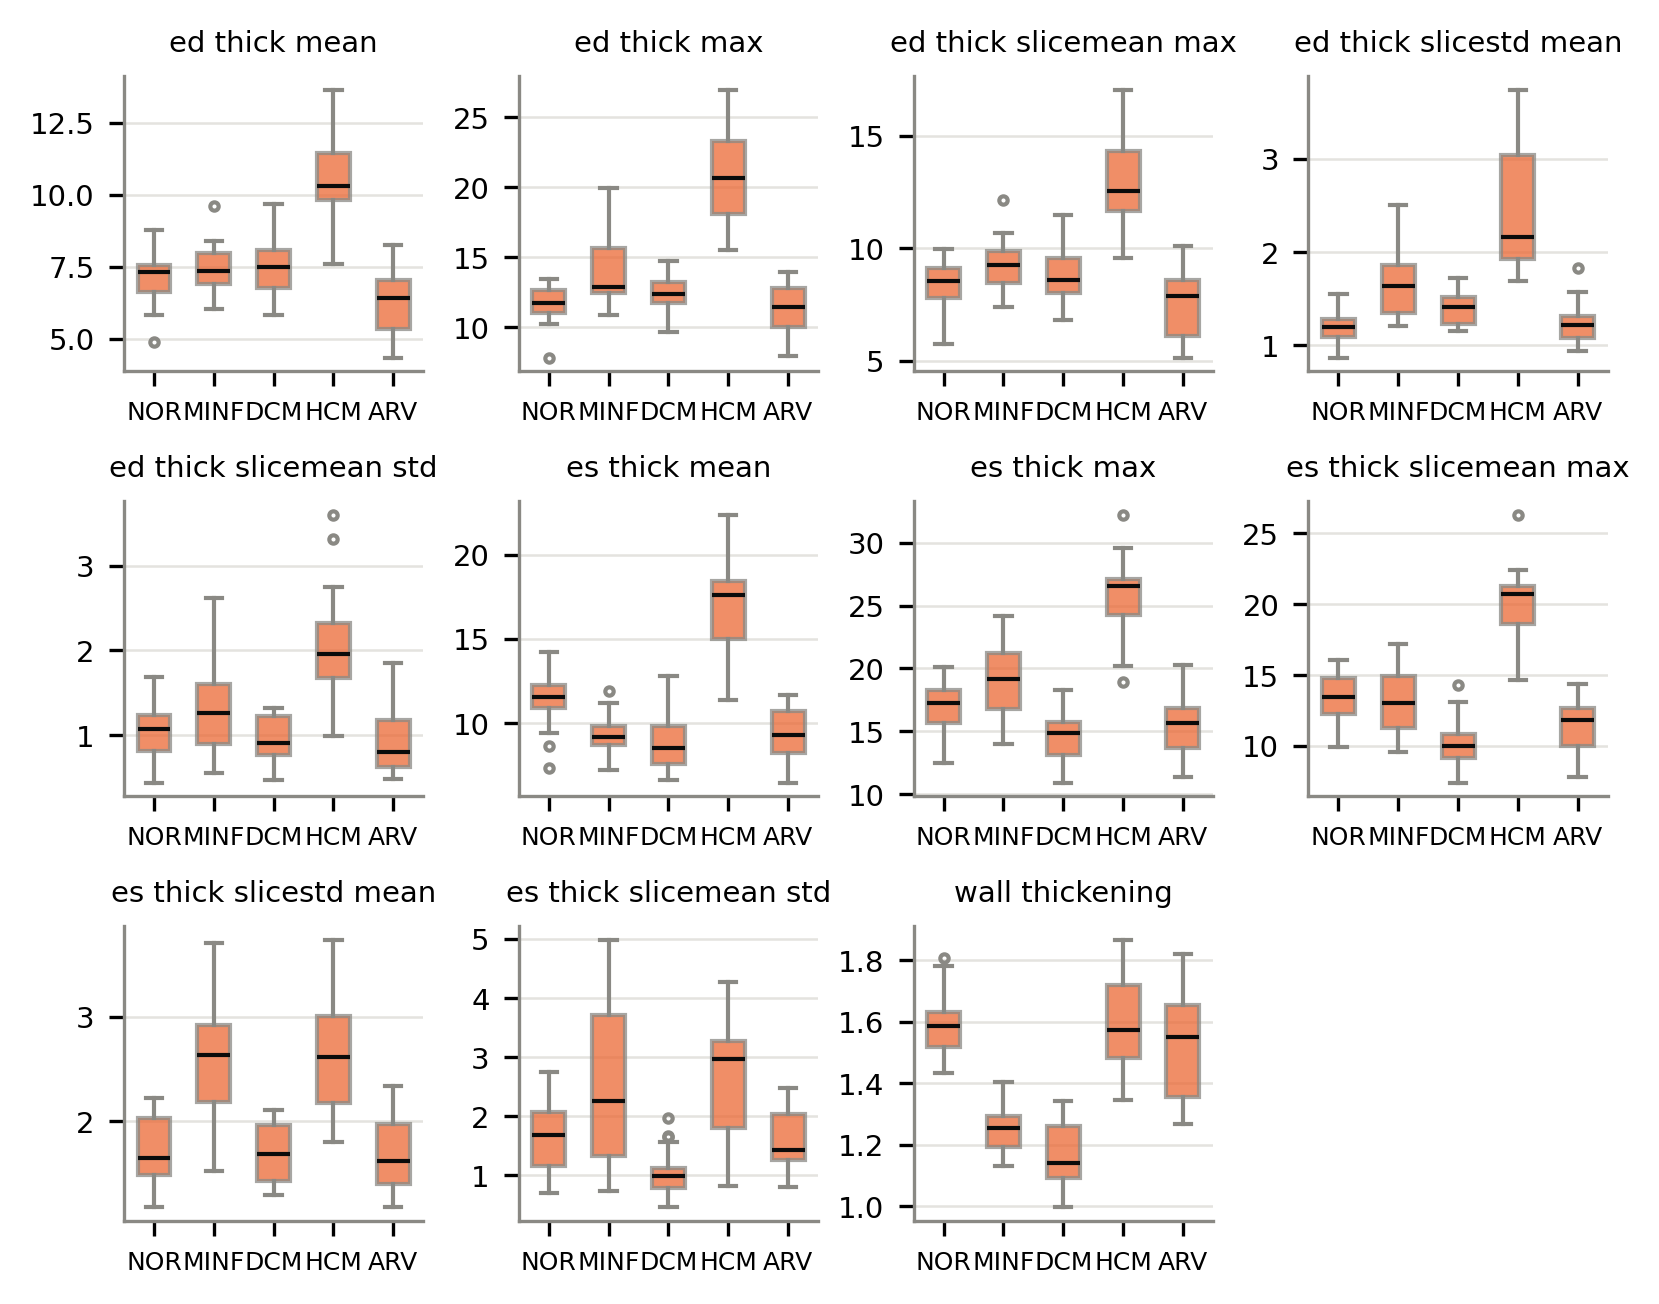
\includegraphics[width=\linewidth]{figs/supp/thickness_by_class.png}
  \caption{Distribution of the 11 thickness features per group (training set, reconstructed LV).}
  \label{fig:supp-thick}
\end{figure}

\clearpage
% ==========================================================================================
\section{Reconstruction of the LV cavity}
\label{app:lv}

\subsection{Volumes not reconstructed exactly}
Table~\ref{tab:supp-lv} lists the 7 training volumes that the filling does not reconstruct exactly. With the convex-hull fallback, the remaining errors are a few boundary voxels of the basal slice (at most 3.1 mL). The filling alone misestimates the ejection fraction of patient 011 by 12 points and of patient 069 by 13 points.

% Generated by regenerate_supplementary.py from results/lv_reconstruction/tables/per_volume.csv
\begin{table}[H]
\centering
\scriptsize
\setlength{\tabcolsep}{4pt}
\begin{adjustbox}{max width=\linewidth}
\begin{tabular}{lllrrrrrrr}
\toprule
Patient & Phase & Class & True LV (mL) & \multicolumn{2}{c}{Filling: $\Delta V$, Dice} & \multicolumn{2}{c}{+ convex hull: $\Delta V$, Dice} & \multicolumn{2}{c}{$\Delta$EF (points)} \\
\midrule
011 & ED & DCM & 237.0 & $-$28.7 & 0.935 & 1.2 & 0.998 & $-$12.1 & 0.4 \\
045 & ES & MINF & 158.6 & $-$25.7 & 0.912 & 1.2 & 0.996 & 11.4 & $-$0.5 \\
029 & ED & HCM & 157.1 & $-$10.8 & 0.965 & 3.1 & 0.990 & $-$1.3 & 0.4 \\
069 & ES & NOR & 33.3 & $-$9.6 & 0.832 & 0.6 & 0.991 & 12.8 & $-$0.8 \\
068 & ES & NOR & 49.3 & $-$9.5 & 0.893 & 0.8 & 0.992 & 7.7 & $-$0.6 \\
096 & ES & ARV & 74.9 & $-$7.3 & 0.949 & 0.4 & 0.998 & 4.8 & $-$0.2 \\
084 & ES & ARV & 22.1 & $-$4.0 & 0.901 & 0.1 & 0.997 & 7.0 & $-$0.2 \\
\bottomrule
\end{tabular}
\end{adjustbox}
\caption{The training volumes that the filling does not reconstruct exactly. Each one misses its most basal slice (slice 0, or 1 for patient 096), where the myocardium does not close around the cavity. The two $\Delta$EF columns are for the filling and for the filling with the convex-hull fallback.}
\label{tab:supp-lv}
\end{table}


\subsection{Effect on the features}
Table~\ref{tab:supp-shift} gives the largest change of each feature when the training LV is reconstructed instead of taken from the ground truth. With the fallback, the volumes and ejection fractions are almost unchanged; the thickness descriptors of the basal slice still change for a few patients, because the reconstructed cavity of that slice is not exactly the true one.

% Generated by regenerate_supplementary.py from results/features/tables/lv_source_shift.csv
\begin{table}[H]
\centering
\small
\setlength{\tabcolsep}{4pt}
\begin{adjustbox}{max width=\linewidth}
\begin{tabular}{lrr}
\toprule
Feature & Filling & + convex hull \\
\midrule
\texttt{stroke\_volume} & 98.5 & 4.0 \\
\texttt{lv\_ef} & 98.3 & 3.5 \\
\texttt{ratio\_rv\_lv\_es} & 40.4 & 1.8 \\
\texttt{es\_lv\_index} & 28.8 & 1.8 \\
\texttt{es\_lv\_vol} & 28.8 & 1.8 \\
\texttt{es\_thick\_slicestd\_mean} & 16.5 & 7.2 \\
\texttt{es\_thick\_slicemean\_std} & 14.5 & 37.5 \\
\texttt{mass\_to\_edv\_ratio} & 13.8 & 1.9 \\
\texttt{ratio\_rv\_lv\_ed} & 13.8 & 1.9 \\
\texttt{myocardium\_to\_lv\_ed} & 13.8 & 1.9 \\
\bottomrule
\end{tabular}
\end{adjustbox}
\caption{Largest relative change (\%, over the 100 training patients) of a feature when the LV is reconstructed instead of taken from the ground truth. Only 7 patients change at all; the ejection fraction of one of them changes by 98\% with the filling.}
\label{tab:supp-shift}
\end{table}


\clearpage
% ==========================================================================================
\section{Protocol study}
\label{app:protocol}

\subsection{Scores of the grids on a single split}
On a single split, most grid configurations obtain the same accuracy, or differ by one patient (Figure~\ref{fig:supp-grid}). The best configuration is therefore determined by one or two patients of one split.

\begin{figure}[H]
  \centering
  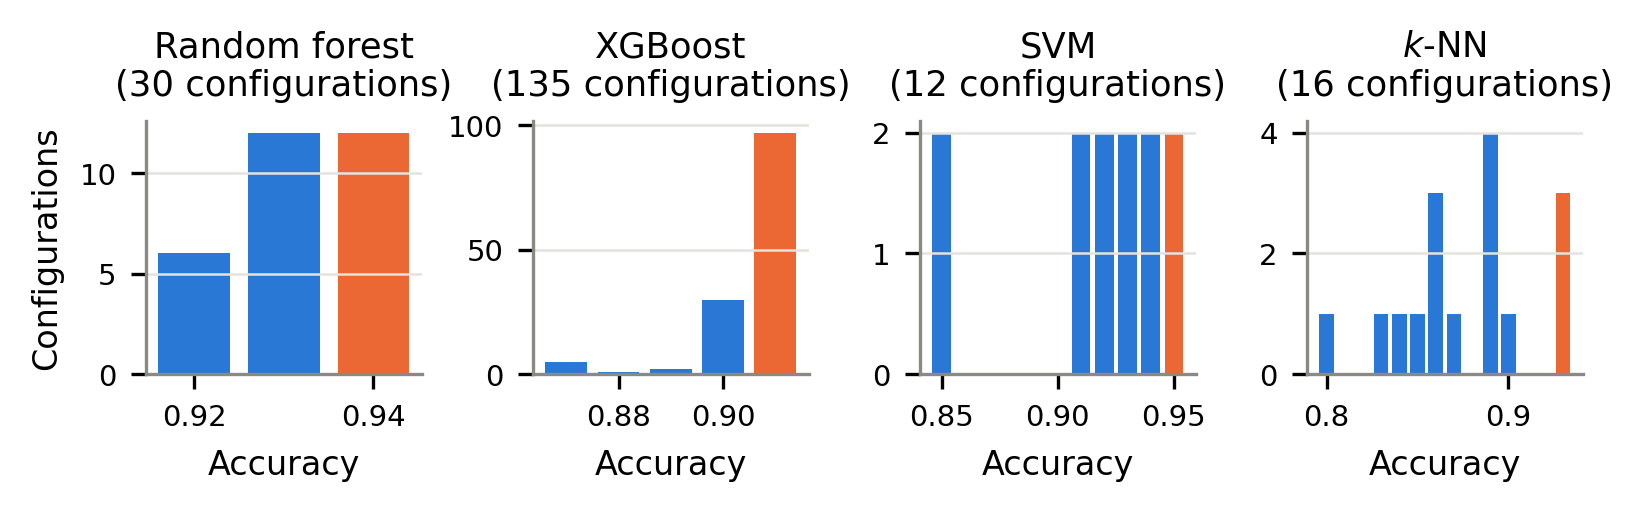
\includegraphics[width=\linewidth]{figs/supp/grid_scores.png}
  \caption{Number of configurations of each grid per accuracy on a single 5-fold split (21 volumetric features, scaler fitted on all patients). Orange: best accuracy, the one a single-split protocol reports.}
  \label{fig:supp-grid}
\end{figure}

\subsection{MLPs scored on their training patients}
Scored on the patients they were trained on, MLP ensembles reach 100\% whatever the number of epochs, so this score cannot select hyper-parameters (Table~\ref{tab:supp-mlp}).

% Generated by regenerate_supplementary.py from results/protocol_study/tables/mlp_training_vs_cv.csv
\begin{table}[H]
\centering
\small
\setlength{\tabcolsep}{4pt}
\begin{adjustbox}{max width=\linewidth}
\begin{tabular}{rrr}
\toprule
Epochs & Accuracy on its training patients & 5-fold CV accuracy \\
\midrule
100 & 1.00 & 0.93 \\
200 & 1.00 & 0.92 \\
500 & 1.00 & 0.93 \\
\bottomrule
\end{tabular}
\end{adjustbox}
\caption{Ensemble of 10 MLPs (same architecture as the final ensemble, learning rate $10^{-3}$, batch 30, 75\% of the patients per MLP), scored on the patients it was trained on and by cross-validation.}
\label{tab:supp-mlp}
\end{table}


\subsection{Feature selection before the cross-validation}
% Generated by regenerate_supplementary.py from results/protocol_study/tables/feature_selection_leak.csv
\begin{table}[H]
\centering
\small
\setlength{\tabcolsep}{4pt}
\begin{adjustbox}{max width=\linewidth}
\begin{tabular}{lr}
\toprule
Random forest (200 trees) & Accuracy \\
\midrule
All 21 features & 0.925 $\pm$ 0.010 \\
Top 16, selected on all patients & 0.924 $\pm$ 0.012 \\
Top 16, selected inside each training fold & 0.923 $\pm$ 0.013 \\
\bottomrule
\end{tabular}
\end{adjustbox}
\caption{Feature selection by random-forest importance, 10 random 5-fold splits (mean $\pm$ std). Selecting on all patients leaks the evaluation folds, but the effect is negligible here.}
\label{tab:supp-selection}
\end{table}


\clearpage
% ==========================================================================================
\section{Benchmark: full results}
\label{app:bench}

\subsection{All configurations}
Table~\ref{tab:supp-benchmark} gives the accuracy, the macro-F1, the recall of each group and the paired difference with the best configuration. NOR is the easiest group (recall 0.95 to 1.00 for almost every model); MINF and DCM are the hardest. The compact set favors HCM and penalizes MINF.

% Generated by regenerate_supplementary.py from results/benchmark/tables/summary_mean.csv
\begin{table}[H]
\centering
\scriptsize
\setlength{\tabcolsep}{4pt}
\begin{adjustbox}{max width=\linewidth}
\begin{tabular}{llrrrrrrrr}
\toprule
Features & Model & Accuracy & Macro-F1 & \multicolumn{5}{c}{Recall: NOR, MINF, DCM, HCM, ARV} & $\Delta$ vs best \\
\midrule
Volumetric & Logistic regression & 0.896 $\pm$ 0.016 & 0.897 & 0.92 & 0.91 & 0.86 & 0.89 & 0.90 & $-$0.070 $\pm$ 0.017 \\
 & Linear SVM & 0.925 $\pm$ 0.016 & 0.925 & 1.00 & 0.94 & 0.86 & 0.87 & 0.94 & $-$0.041 $\pm$ 0.019 \\
 & RBF SVM & 0.923 $\pm$ 0.022 & 0.923 & 0.94 & 0.94 & 0.91 & 0.91 & 0.92 & $-$0.043 $\pm$ 0.025 \\
 & $k$-NN & 0.895 $\pm$ 0.010 & 0.897 & 1.00 & 0.92 & 0.89 & 0.87 & 0.80 & $-$0.071 $\pm$ 0.014 \\
 & Random forest & 0.923 $\pm$ 0.016 & 0.923 & 0.97 & 0.88 & 0.89 & 0.94 & 0.94 & $-$0.043 $\pm$ 0.018 \\
 & Extra trees & 0.931 $\pm$ 0.010 & 0.931 & 0.99 & 0.92 & 0.91 & 0.93 & 0.91 & $-$0.035 $\pm$ 0.012 \\
 & XGBoost & 0.920 $\pm$ 0.013 & 0.920 & 0.96 & 0.88 & 0.91 & 0.94 & 0.91 & $-$0.046 $\pm$ 0.014 \\
 & MLP ensemble & 0.920 $\pm$ 0.012 & 0.921 & 0.97 & 0.94 & 0.89 & 0.89 & 0.91 & $-$0.046 $\pm$ 0.014 \\
 & MLP + RF & 0.925 $\pm$ 0.012 & 0.926 & 1.00 & 0.93 & 0.88 & 0.91 & 0.92 & $-$0.041 $\pm$ 0.014 \\
 & MLP + linear SVM & 0.927 $\pm$ 0.012 & 0.928 & 0.99 & 0.94 & 0.88 & 0.91 & 0.91 & $-$0.039 $\pm$ 0.014 \\
\midrule
Volumetric + thickness & Logistic regression & 0.953 $\pm$ 0.014 & 0.953 & 0.99 & 0.95 & 0.95 & 0.94 & 0.93 & $-$0.013 $\pm$ 0.015 \\
 & Linear SVM & 0.956 $\pm$ 0.014 & 0.956 & 0.97 & 0.95 & 0.93 & 0.97 & 0.94 & $-$0.010 $\pm$ 0.009 \\
 & RBF SVM & 0.945 $\pm$ 0.012 & 0.945 & 0.95 & 0.94 & 0.93 & 0.97 & 0.94 & $-$0.021 $\pm$ 0.013 \\
 & $k$-NN & 0.902 $\pm$ 0.023 & 0.903 & 0.98 & 0.91 & 0.90 & 0.92 & 0.80 & $-$0.064 $\pm$ 0.029 \\
 & Random forest & 0.938 $\pm$ 0.015 & 0.938 & 1.00 & 0.90 & 0.91 & 0.95 & 0.93 & $-$0.028 $\pm$ 0.017 \\
 & Extra trees & 0.937 $\pm$ 0.012 & 0.937 & 0.99 & 0.91 & 0.94 & 0.95 & 0.90 & $-$0.029 $\pm$ 0.015 \\
 & XGBoost & 0.916 $\pm$ 0.021 & 0.916 & 0.99 & 0.86 & 0.91 & 0.94 & 0.89 & $-$0.050 $\pm$ 0.022 \\
 & MLP ensemble & 0.957 $\pm$ 0.008 & 0.957 & 0.99 & 0.95 & 0.93 & 0.95 & 0.95 & $-$0.009 $\pm$ 0.008 \\
 & MLP + RF & 0.954 $\pm$ 0.010 & 0.954 & 1.00 & 0.95 & 0.93 & 0.95 & 0.94 & $-$0.012 $\pm$ 0.012 \\
 & MLP + linear SVM & 0.966 $\pm$ 0.011 & 0.966 & 0.98 & 0.95 & 0.94 & 0.97 & 0.97 & 0.000 $\pm$ 0.000 \\
\midrule
Compact & Logistic regression & 0.942 $\pm$ 0.015 & 0.942 & 0.99 & 0.89 & 0.89 & 1.00 & 0.94 & $-$0.024 $\pm$ 0.015 \\
 & Linear SVM & 0.927 $\pm$ 0.009 & 0.927 & 1.00 & 0.91 & 0.85 & 0.95 & 0.93 & $-$0.039 $\pm$ 0.009 \\
 & RBF SVM & 0.944 $\pm$ 0.019 & 0.944 & 0.99 & 0.89 & 0.91 & 1.00 & 0.93 & $-$0.022 $\pm$ 0.021 \\
 & $k$-NN & 0.932 $\pm$ 0.012 & 0.932 & 0.99 & 0.90 & 0.97 & 0.96 & 0.83 & $-$0.034 $\pm$ 0.015 \\
 & Random forest & 0.925 $\pm$ 0.019 & 0.925 & 1.00 & 0.88 & 0.88 & 0.98 & 0.89 & $-$0.041 $\pm$ 0.022 \\
 & Extra trees & 0.940 $\pm$ 0.009 & 0.940 & 0.99 & 0.91 & 0.94 & 0.99 & 0.86 & $-$0.026 $\pm$ 0.014 \\
 & XGBoost & 0.915 $\pm$ 0.022 & 0.915 & 0.98 & 0.88 & 0.88 & 0.98 & 0.85 & $-$0.051 $\pm$ 0.023 \\
 & MLP ensemble & 0.953 $\pm$ 0.014 & 0.953 & 1.00 & 0.90 & 0.93 & 0.99 & 0.94 & $-$0.013 $\pm$ 0.018 \\
 & MLP + RF & 0.952 $\pm$ 0.019 & 0.952 & 1.00 & 0.90 & 0.93 & 0.98 & 0.94 & $-$0.014 $\pm$ 0.023 \\
 & MLP + linear SVM & 0.955 $\pm$ 0.008 & 0.955 & 1.00 & 0.91 & 0.92 & 0.98 & 0.97 & $-$0.011 $\pm$ 0.014 \\
\bottomrule
\end{tabular}
\end{adjustbox}
\caption{All configurations of the benchmark (nested CV, 10 repeats, reconstructed LV). $\Delta$ vs best: per-repeat difference with the best configuration (MLP + linear SVM, volumetric + thickness), mean $\pm$ std; since all configurations share the same splits, this paired difference is less noisy than the accuracies themselves.}
\label{tab:supp-benchmark}
\end{table}


\subsection{Recall per group}
\begin{figure}[H]
  \centering
  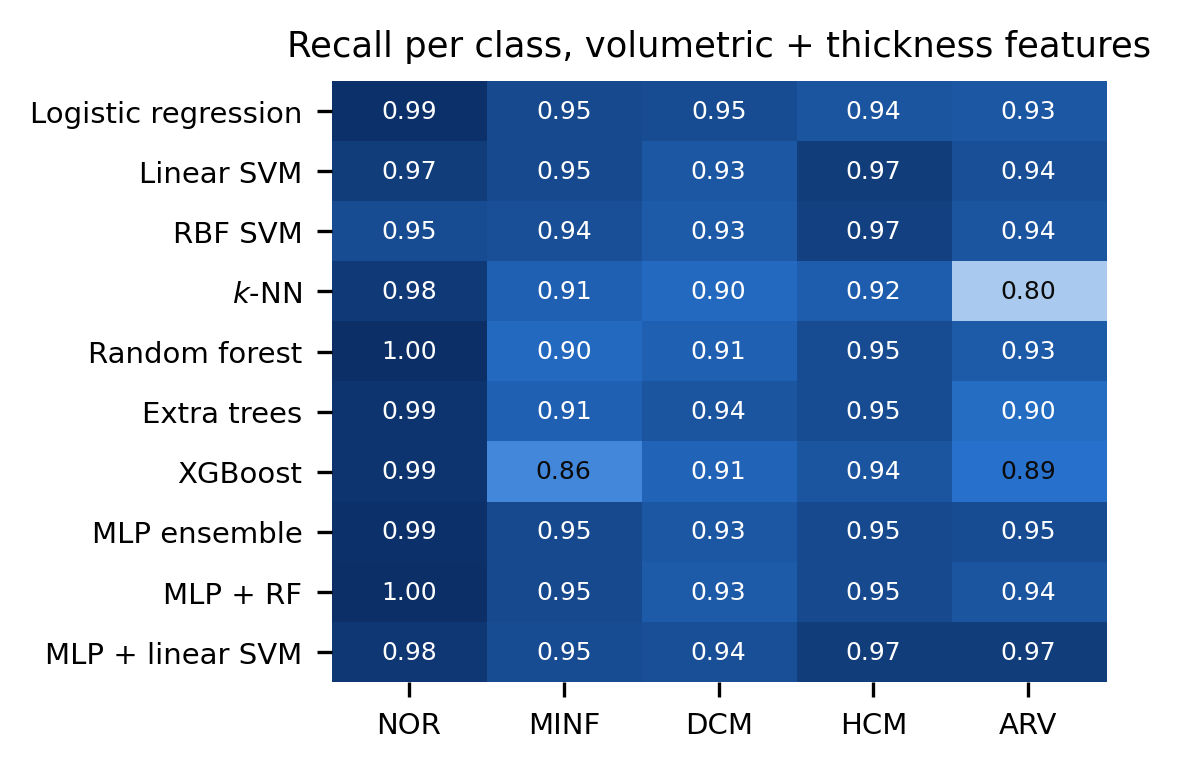
\includegraphics[width=0.62\linewidth]{figs/supp/recall_heatmap.png}
  \caption{Recall of each group for the 10 classifiers on the 32 features (volumetric + thickness).}
  \label{fig:supp-recall}
\end{figure}

\subsection{Hyper-parameters}
The inner cross-validation chooses stable values for the forests (fully grown trees, $\sqrt{d}$ features per split) and XGBoost (shallow trees, column subsampling), and less stable ones for the regularization of the linear models, whose accuracy is flat over a wide range of $C$ (Table~\ref{tab:supp-hyper}). For the soft votes, $\alpha=0.5$ is the most frequent choice, but in less than half of the folds for 5 of the 6 ensembles: this suggests that the inner cross-validation often finds several values of $\alpha$ tied, the tie-breaking rule then picking 0.5.

% Generated by regenerate_supplementary.py from results/benchmark/tables/summary.csv
\begin{table}[H]
\centering
\scriptsize
\setlength{\tabcolsep}{4pt}
\begin{adjustbox}{max width=\linewidth}
\begin{tabular}{llp{0.58\linewidth}}
\toprule
Features & Model & Most frequent choice of the inner CV (count over the 50 outer folds) \\
\midrule
Volumetric & Logistic regression & C=0.01 (14/50) \\
Volumetric & Linear SVM & C=0.1 (33/50) \\
Volumetric & RBF SVM & C=10 (27/50), gamma=scale (25/50) \\
Volumetric & $k$-NN & metric=manhattan (47/50), n\_neighbors=3 (26/50), weights=distance (31/50) \\
Volumetric & Random forest & max\_depth=None (48/50), max\_features=sqrt (43/50) \\
Volumetric & Extra trees & max\_depth=None (37/50), max\_features=sqrt (33/50) \\
Volumetric & XGBoost & colsample\_bytree=0.6 (47/50), learning\_rate=0.05 (44/50), max\_depth=2 (30/50), n\_estimators=100 (35/50) \\
Volumetric & MLP + RF & alpha=0.5 (19/50) \\
Volumetric & MLP + linear SVM & alpha=0.5 (24/50) \\
Volumetric + thickness & Logistic regression & C=10.0 (16/50) \\
Volumetric + thickness & Linear SVM & C=0.1 (32/50) \\
Volumetric + thickness & RBF SVM & C=10 (27/50), gamma=scale (30/50) \\
Volumetric + thickness & $k$-NN & metric=manhattan (29/50), n\_neighbors=5 (15/50), weights=distance (30/50) \\
Volumetric + thickness & Random forest & max\_depth=None (44/50), max\_features=sqrt (44/50) \\
Volumetric + thickness & Extra trees & max\_depth=None (29/50), max\_features=sqrt (38/50) \\
Volumetric + thickness & XGBoost & colsample\_bytree=0.6 (46/50), learning\_rate=0.05 (36/50), max\_depth=2 (35/50), n\_estimators=100 (25/50) \\
Volumetric + thickness & MLP + RF & alpha=0.5 (21/50) \\
Volumetric + thickness & MLP + linear SVM & alpha=0.5 (33/50) \\
Compact & Logistic regression & C=0.1 (15/50) \\
Compact & Linear SVM & C=1.0 (19/50) \\
Compact & RBF SVM & C=1 (24/50), gamma=scale (36/50) \\
Compact & $k$-NN & metric=euclidean (43/50), n\_neighbors=3 (39/50), weights=distance (30/50) \\
Compact & Random forest & max\_depth=None (45/50), max\_features=sqrt (45/50) \\
Compact & Extra trees & max\_depth=None (32/50), max\_features=sqrt (41/50) \\
Compact & XGBoost & colsample\_bytree=0.6 (47/50), learning\_rate=0.05 (42/50), max\_depth=3 (25/50), n\_estimators=100 (27/50) \\
Compact & MLP + RF & alpha=0.5 (18/50) \\
Compact & MLP + linear SVM & alpha=0.5 (21/50) \\
\bottomrule
\end{tabular}
\end{adjustbox}
\caption{Hyper-parameters selected by the inner cross-validation. Grids: $C\in\{0.01,0.1,1,10,100\}$ for logistic regression and the linear SVM; $C\in\{0.1,1,10,100\}$, $\gamma\in\{$scale$, 0.01, 0.1\}$ for the RBF SVM; $k\in\{3,5,7,9\}$, uniform or distance weights, Euclidean or Manhattan for $k$-NN; depth $\in\{$none$, 5\}$, features per split $\in\{\sqrt{d}, d/2\}$ for the forests (300 trees); 100 or 300 trees, depth 2 or 3, learning rate 0.05 or 0.1, column subsampling 0.6 or 1 for XGBoost; $\alpha\in\{0,0.1,\dots,1\}$ for the soft votes. A frequent \texttt{None} depth means fully grown trees.}
\label{tab:supp-hyper}
\end{table}


\clearpage
% ==========================================================================================
\section{Final model}
\label{app:final}

\subsection{Repeats and errors}
% Generated by regenerate_supplementary.py from results/final_model/tables/nested_per_repeat.csv
\begin{table}[H]
\centering
\small
\setlength{\tabcolsep}{4pt}
\begin{adjustbox}{max width=\linewidth}
\begin{tabular}{rrrrrrr}
\toprule
Repeat & Accuracy & NOR & MINF & DCM & HCM & ARV \\
\midrule
0 & 0.98 & 1.00 & 0.95 & 0.95 & 1.00 & 1.00 \\
1 & 0.96 & 0.95 & 0.95 & 0.95 & 0.95 & 1.00 \\
2 & 0.97 & 1.00 & 0.95 & 0.95 & 0.95 & 1.00 \\
3 & 0.97 & 1.00 & 0.95 & 0.95 & 1.00 & 0.95 \\
4 & 0.97 & 0.95 & 0.95 & 0.95 & 1.00 & 1.00 \\
5 & 0.96 & 1.00 & 0.95 & 1.00 & 0.95 & 0.90 \\
6 & 0.97 & 1.00 & 0.95 & 0.95 & 0.95 & 1.00 \\
7 & 0.94 & 0.95 & 0.95 & 0.90 & 0.95 & 0.95 \\
8 & 0.97 & 1.00 & 0.95 & 0.90 & 1.00 & 1.00 \\
9 & 0.97 & 1.00 & 0.95 & 0.95 & 1.00 & 0.95 \\
\midrule
Mean & 0.966 $\pm$ 0.011 & 0.985 & 0.950 & 0.945 & 0.975 & 0.975 \\
\bottomrule
\end{tabular}
\end{adjustbox}
\caption{Final model, nested CV: accuracy and recall per class for each of the 10 repeats (100 patients each).}
\label{tab:supp-repeats}
\end{table}

% Generated by regenerate_supplementary.py from results/final_model/tables/misclassified_patients.csv
\begin{table}[H]
\centering
\small
\setlength{\tabcolsep}{4pt}
\begin{adjustbox}{max width=\linewidth}
\begin{tabular}{lllrrrrr}
\toprule
Patient & True & Most predicted & Error rate & LV EF & LV EDV / BSA & ES thick.\ std & RV EF \\
\midrule
050 & MINF & DCM & 1.0 & 16.4 & 162.5 & 2.18 & 72.5 \\
002 & DCM & MINF & 0.9 & 29.1 & 150.7 & 2.06 & 69.5 \\
022 & HCM & HCM & 0.5 & 64.9 & 51.7 & 1.89 & 44.2 \\
015 & DCM & DCM & 0.2 & 25.7 & 123.2 & 1.34 & 46.8 \\
067 & NOR & NOR & 0.2 & 59.7 & 83.6 & 1.50 & 49.3 \\
088 & ARV & ARV & 0.2 & 48.4 & 78.7 & 2.33 & 44.6 \\
089 & ARV & ARV & 0.2 & 62.8 & 34.9 & 1.60 & 10.1 \\
065 & NOR & NOR & 0.1 & 66.0 & 67.9 & 2.07 & 60.7 \\
082 & ARV & ARV & 0.1 & 55.0 & 70.6 & 2.12 & 45.0 \\
\bottomrule
\end{tabular}
\end{adjustbox}
\caption{Patients misclassified in at least one of the 10 repeats of the final model, with four of their features (class means in Table~\ref{tab:supp-features}).}
\label{tab:supp-errors}
\end{table}


\subsection{Permutation importance}
% Generated by regenerate_supplementary.py from results/final_model/tables/permutation_importance.csv
\begin{table}[H]
\centering
\scriptsize
\setlength{\tabcolsep}{4pt}
\begin{adjustbox}{max width=\linewidth}
\begin{tabular}{lrlr}
\toprule
Feature & Accuracy drop & Feature & Accuracy drop \\
\midrule
\texttt{es\_thick\_slicestd\_mean} & 0.050 $\pm$ 0.033 & \texttt{ed\_rv\_vol} & 0.007 $\pm$ 0.015 \\
\texttt{lv\_ef} & 0.025 $\pm$ 0.016 & \texttt{ed\_lv\_index} & 0.006 $\pm$ 0.015 \\
\texttt{rv\_ef} & 0.024 $\pm$ 0.033 & \texttt{es\_thick\_mean} & 0.005 $\pm$ 0.017 \\
\texttt{stroke\_volume} & 0.024 $\pm$ 0.029 & \texttt{es\_thick\_slicemean\_max} & 0.005 $\pm$ 0.020 \\
\texttt{es\_rv\_vol} & 0.019 $\pm$ 0.023 & \texttt{ed\_rv\_index} & 0.005 $\pm$ 0.016 \\
\texttt{ratio\_rv\_lv\_es} & 0.019 $\pm$ 0.023 & \texttt{es\_lv\_index} & 0.005 $\pm$ 0.011 \\
\texttt{myocardium\_mass} & 0.018 $\pm$ 0.024 & \texttt{ed\_thick\_slicemean\_std} & 0.005 $\pm$ 0.015 \\
\texttt{height} & 0.017 $\pm$ 0.018 & \texttt{mass\_to\_edv\_ratio} & 0.004 $\pm$ 0.015 \\
\texttt{lv\_mass\_index} & 0.016 $\pm$ 0.017 & \texttt{es\_thick\_max} & 0.003 $\pm$ 0.024 \\
\texttt{ratio\_rv\_lv\_ed} & 0.015 $\pm$ 0.018 & \texttt{es\_lv\_vol} & 0.003 $\pm$ 0.007 \\
\texttt{es\_rv\_index} & 0.014 $\pm$ 0.026 & \texttt{myocardium\_to\_lv\_ed} & 0.002 $\pm$ 0.016 \\
\texttt{ed\_thick\_max} & 0.013 $\pm$ 0.025 & \texttt{ed\_thick\_mean} & 0.001 $\pm$ 0.021 \\
\texttt{es\_thick\_slicemean\_std} & 0.012 $\pm$ 0.020 & \texttt{ed\_thick\_slicemean\_max} & $-$0.001 $\pm$ 0.011 \\
\texttt{ed\_lv\_vol} & 0.011 $\pm$ 0.021 & \texttt{bsa} & $-$0.001 $\pm$ 0.018 \\
\texttt{wall\_thickening} & 0.011 $\pm$ 0.015 & \texttt{weight} & $-$0.003 $\pm$ 0.012 \\
\texttt{ed\_thick\_slicestd\_mean} & 0.010 $\pm$ 0.026 & \texttt{mass\_ratio\_systole\_diastole} & $-$0.003 $\pm$ 0.017 \\
\bottomrule
\end{tabular}
\end{adjustbox}
\caption{Permutation importance of every feature for the final model: drop of held-out accuracy when the feature is shuffled (20 permutations, 15 folds of 3 repeated 5-fold CVs; mean $\pm$ std over folds). Correlated features share their importance, so low values do not mean the information is useless.}
\label{tab:supp-importance}
\end{table}


\subsection{Test predictions}
The predicted groups are close to balanced, and most test patients are predicted with a probability above 0.7 (Figure~\ref{fig:supp-test}).

\begin{figure}[H]
  \centering
  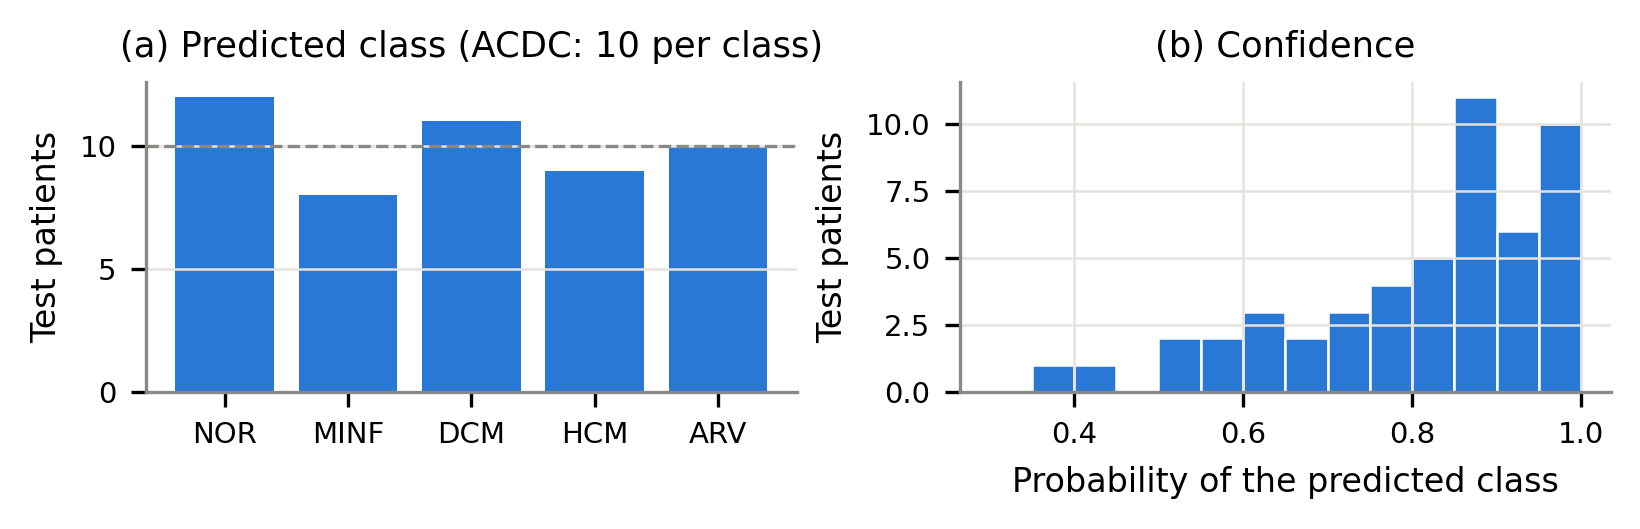
\includegraphics[width=\linewidth]{figs/supp/test_predictions.png}
  \caption{(a) Number of test patients predicted in each group by the final model; the dashed line marks the 10 patients per group of the ACDC test set. (b) Distribution of the probability of the predicted group.}
  \label{fig:supp-test}
\end{figure}

\clearpage
% ==========================================================================================
\section{Reproducibility}
\label{app:runs}

\subsection{Code organization}
The code is a Python package (data access, LV reconstruction, features, models, nested cross-validation, experiment tracking, figures) and six scripts run in order. Every run creates a timestamped folder with the configuration, library versions, log, metrics, tables (CSV and \LaTeX), figures and out-of-fold predictions; the latest successful run of each experiment is kept for the report. The data folders are only read.

\subsection{Experiments and running times}
% Generated by regenerate_supplementary.py from results/runs.csv
\begin{table}[H]
\centering
\small
\setlength{\tabcolsep}{4pt}
\begin{adjustbox}{max width=\linewidth}
\begin{tabular}{lcr}
\toprule
Experiment & Script & Time (min) \\
\midrule
Patient index, file checks & 1 & 0.1 \\
LV reconstruction on the training set & 2 & 0.3 \\
Features for every LV source & 3 & 0.7 \\
Protocol study (single split vs nested CV) & 4 & 14.3 \\
Benchmark (30 configurations, nested CV) & 5 & 48.8 \\
LV protocols (32 configurations) & 5 & 17.6 \\
Final model and test predictions & 6 & 6.9 \\
\bottomrule
\end{tabular}
\end{adjustbox}
\caption{Runs that produced the results of this report (Apple M3, 16 GB, 8 CPU cores; no GPU). Most of the time is spent training MLP ensembles inside the nested cross-validation.}
\label{tab:supp-runs}
\end{table}


\subsection{Software and parameters}
Python 3.12.6, NumPy 2.2.6, pandas 2.2.3, SciPy 1.14.1, scikit-learn 1.5.2, scikit-image 0.24.0, nibabel 5.3.2, PyTorch 2.6.0, XGBoost 3.0.0. Outer cross-validation: stratified 5-fold, 10 repeats (5 for the protocol study), seeds 0 to 9 (42 to 46 for the protocol study). Inner cross-validation: stratified 5-fold, accuracy as selection criterion, first configuration kept in case of ties (closest to 0.5 for $\alpha$). Logistic regression: multinomial, L2 penalty. SVMs: probabilities by Platt scaling with an internal 5-fold cross-validation. Random forests and extra trees: 300 trees. MLP ensemble: 50 networks, layer widths $d \to 32 \to 32 \to 32 \to 32 \to 5$, batch normalization (momentum 0.1), leaky ReLU (slope 0.01), cross-entropy, Adam with learning rate $10^{-3}$, 200 epochs, batches of 30, 75\% of the patients and $\lfloor 2d/3\rfloor$ features per network.

\stopcontents[appendix]


\end{document}
